\documentclass[final,5p,times,twocolumn]{elsarticle}

\usepackage{amsmath}
\usepackage{amssymb}
\usepackage{booktabs}
\usepackage{multirow}
\usepackage{graphicx}
% Figures live in figures/ locally; Editorial Manager flattens all
% uploaded files into one directory. Search both.
\graphicspath{{figures/}{./}}
\usepackage{subcaption}
\usepackage{url}
\usepackage{hyperref}
\hypersetup{hidelinks,
  pdfauthor={}, pdftitle={}, pdfsubject={}, pdfkeywords={}, pdfcreator={}}
\usepackage{xurl} % allow long URLs to break across lines
\usepackage{placeins}
\usepackage{dblfloatfix}
\usepackage{float}
\usepackage{tabularx}
\usepackage{array}
\usepackage{etoolbox}
% Compact bibliography to meet the 18-page submission limit.
\AtBeginEnvironment{thebibliography}{\footnotesize}

\journal{Future Generation Computer Systems}

% Float tuning: avoid a large figure* being exiled to a mostly-empty
% float page; prefer top-of-page placement with text flowing beneath.
\renewcommand{\dbltopfraction}{0.95}
\renewcommand{\dblfloatpagefraction}{0.9}
\setcounter{dbltopnumber}{2}
\renewcommand{\topfraction}{0.9}
\renewcommand{\textfraction}{0.07}
\renewcommand{\floatpagefraction}{0.85}
\setlength{\floatsep}{7pt plus 2pt minus 2pt}
\setlength{\textfloatsep}{9pt plus 2pt minus 3pt}
\setlength{\intextsep}{8pt plus 2pt minus 2pt}
\setlength{\dblfloatsep}{7pt plus 2pt minus 2pt}
\setlength{\dbltextfloatsep}{9pt plus 2pt minus 3pt}
\setlength{\abovecaptionskip}{4pt}
\setlength{\belowcaptionskip}{2pt}
\AtBeginDocument{\ifdefined\bibsep\setlength{\bibsep}{1pt plus 0.2ex}\fi}

\begin{document}

\begin{frontmatter}

\title{Conversational Counterfactual Guidance for Operator-Centred
Hyperparameter Optimisation in Industrial Anomaly Detection}

%% ---------------------------------------------------------------
%% Author names, affiliations, corresponding-author details and the
%% CRediT statement have been removed for double-blind review and are
%% supplied in the separate title page file.
%% ---------------------------------------------------------------

\begin{abstract}
Hyperparameter optimisation (HPO) logs are rarely reused for interpretation, although industrial anomaly detection trades detection quality against training data, review effort, and data quality. Counterfactual Explainable HPO (CF-XHPO) reuses trials to train a surrogate and generate constrained what-if recommendations through a schema-constrained conversational interface. We separate surrogate-level query satisfaction from main-model confirmation by retraining PatchCore under three seeds for 24 recommendations each on the MVTec Anomaly Detection benchmark and the Proditec production dataset. All 48 satisfy their surrogate queries and meet their targets after retraining when confirmation follows the per-category
protocol of the optimisation objective (mean confirmed F1 0.879 on
Proditec, gap $-0.007$; 0.787 on MVTec, gap $-0.023$). The MVTec result validates the protocol, not the recommendations: its objective is degenerate at the HPO budget (validation F1 0.58 for a random and 0.83 for a perfect ranker, top tenth of the log within 0.80--0.82), an untuned PatchCore reference beats the HPO optimum (0.867 vs 0.786, one seed), and pooling heterogeneous categories drives AUROC from 0.91 to 0.53.
Constrained retrieval matches off-log generation and a filter-and-sort
baseline, so dense logs need no surrogate for retrieval. A 22-participant study finds high task validity in both workflows; questionnaire differences are descriptive. The study-time parser parsed 15\% of benchmark utterances exactly on the fields the interface uses, and 25 of 72 live parses were incomplete or unfaithful, 8 shown as fluent lists; the study thus evaluates the repair-and-iteration workflow; deterministic resolution of relative constraints is the immediate requirement.
\end{abstract}

\begin{keyword}
hyperparameter optimisation \sep counterfactual explanations \sep
anomaly detection \sep conversational interface \sep explainable artificial intelligence
\sep industrial decision support
\end{keyword}

\end{frontmatter}

% =======================================================================
\section{Introduction}
\label{sec:introduction}
% =======================================================================

Industrial visual inspection increasingly relies on machine-learning
models to detect defects, reduce manual inspection effort, and support
more consistent quality-control decisions. Deep learning has driven
rapid progress in this area \cite{xie_deep_2024}, with benchmarks and
methods such as the MVTec Anomaly Detection (MVTec~AD) benchmark,
PatchCore, and EfficientAD among the most
widely used reference points
\cite{bergmann_mvtec_2019,roth_towards_2022,batzner_efficientad_2024}.
In this setting, however, a useful model is not defined by detection
performance alone. Engineers and operators must also consider practical
constraints such as the amount of training data available, the expected
review effort, the quality of the input data, and the cost of
retraining or deploying a new configuration. Hyperparameter
optimisation (HPO) is therefore not only a technical search problem,
but also a decision-support problem in which different configurations
represent different operational trade-offs.

Automated HPO frameworks explore large configuration spaces
effectively \cite{10.1145/3292500.3330701,eggensperger_hpobench_2021},
but their outputs are ranked configurations, optimisation traces,
visual analytics, or importance summaries
\cite{NEURIPS2021_12ced2db,zoller_xautoml_2023,mu_shrinkhpo_2024}. These
show which configurations performed well, not what should change if the
operator wants similar quality with less review effort, a lower
training fraction, or better robustness to data corruption, which is
how industrial users reason: in constraints and preferences rather
than low-level hyperparameters.

This paper addresses this problem by proposing Counterfactual Explainable
Hyperparameter Optimisation (CF-XHPO), a framework that turns HPO logs
into an interactive recommendation layer. Instead of discarding
optimisation trials once the best configuration is found, CF-XHPO uses
the log to train a surrogate of the configuration--performance
relationship and to retrieve or generate alternatives under new
operator constraints. The surrogate provides a millisecond-scale
screening layer; main-model confirmation remains the final evidence for
a selected configuration. On top of this layer, the framework compares
complementary counterfactual-generation methods with constrained log
retrieval, building on work on diverse, feasible, and actionable
counterfactual explanations
\cite{10.1145/3351095.3372850,dandl_multiobjective_2020,poyiadzi_face_2020,DEOLIVEIRA2023}.
These alternatives respect a separation between hard model
hyperparameters and soft operator-facing controls, so recommendations
stay technically valid while remaining expressed in terms operators can
act on. To support such interaction, CF-XHPO includes a schema-constrained
conversational layer, motivated by recent work on natural-language
model explanation and conversational explainable artificial
intelligence (XAI)
\cite{slack_explaining_2023,liao_questioning_2020,he_is_2025}, through
which operators can state goals in plain language, compare ranked
alternatives, and receive concise explanations of the main
trade-offs.



We evaluate the framework on the MVTec benchmark and the Proditec
industrial inspection use case with the same PatchCore pipeline and
configuration space, retraining every primary recommendation with the
underlying model so that query satisfaction under the surrogate can be
separated from confirmed quality.

Manai et al.\ \cite{manai_cfhpo_conference} demonstrated
soft-control-constrained counterfactual guidance on tabular
classification benchmarks. The present paper extends that work,
retaining its hard/soft control separation and log-reuse idea and
rebuilding the remainder for industrial visual anomaly detection. Its main contributions are a two-dataset industrial evaluation with over 500 PatchCore retrainings: the 48 primary recommendations under three seeds, a five-anchor sweep, a retrieval baseline, 96 logged trials, and a no-HPO reference; a protocol-level analysis showing that confirmation must follow the optimisation objective (per-category models and thresholds), that pooling heterogeneous categories destroys the score ranking, and that the MVTec review-budget objective is degenerate at the HPO budget, so that MVTec supports protocol and objective lessons rather than a claim of recommendation value; and a
schema-constrained conversational layer with workflow evaluation
covering factual-anchor sensitivity, constrained retrieval,
multi-alternative runtime, a labelled parser test, and a 22-participant
study (Sections~\ref{subsec:gap-diagnosis}--\ref{sec:user-study}).
Section~\ref{subsec:rw-conference} sets out the comparison in full.

The evaluation asks three questions: (Q1)~whether a recommendation
that satisfies its query under the surrogate also meets the target
when the underlying model is retrained, and under which confirmation
protocol; (Q2)~when retrieval from the existing log suffices and when
generation beyond it adds coverage or confirmed quality; and
(Q3)~whether technically literate users can act on the alternatives
through the conversational workflow, and how much of that outcome is
due to the parser rather than to repair and iteration.

% =======================================================================
\section{Related Work}
\label{sec:related-work}
% =======================================================================

The proposed framework sits at the intersection of four research
threads: explainable HPO, counterfactual explanations, conversational
XAI, and industrial anomaly detection. This section reviews each
thread and explains how they combine in our work.

\subsection{Explainable and Interactive Hyperparameter Optimisation}
\label{subsec:rw-xhpo}

Hyperparameter optimisation (HPO) is central to modern
machine-learning workflows. Frameworks such as Optuna provide flexible black-box search over large spaces while recording trial-level results \cite{10.1145/3292500.3330701}. Their
outputs, however, are optimisation traces, best-trial summaries, or
ranked configurations: dashboards and visual-analytics tools such as
XAutoML \cite{zoller_xautoml_2023} show \emph{which} configurations
performed well, not \emph{how} a configuration should change to meet a
new operator constraint, and surrogate-based importance analysis
\cite{theodorakopoulos_hyperparameter_2024} serves benchmarking rather
than user-facing recommendation. Shapley-based hyperparameter importance
has recently been extended to feature interactions
\cite{wever2025hypershap}, and large language models are being used to
drive or explain AutoML and HPO
\cite{tornede2024automl,liu2024llambo,zhang2024llmhpo}; these works
explain or automate the search itself, whereas we reuse its finished
log for post-hoc operator guidance.

A parallel effort makes HPO and automated machine learning (AutoML)
more transparent: partial
dependence plots explain hyperparameter effects across the explored
space \cite{NEURIPS2021_12ced2db}, ShrinkHPO exposes and prunes less
promising search regions \cite{mu_shrinkhpo_2024}, and explainable Bayesian optimisation targets users who need to understand the search process itself \cite{10.1007/978-3-032-08324-1_3}.

Together, these works establish that transparency, interaction, and
surrogate modelling matter in HPO and AutoML, but they mainly support
optimisation analysis, benchmarking, or visual inspection rather than
post-hoc configuration guidance under user-defined practical
constraints. Surrogate modelling of nonlinear response surfaces itself
draws on a broad applied literature in which Gaussian-process
regression, graphical and causal models, neural networks, and
composite forecasts are used to capture complicated nonlinear patterns
across application domains
\cite{jin2024gpr,jin2026dag,jin2025nn,xu2021composite};
Section~\ref{subsec:surrogate-fidelity} compares our gradient-boosted
surrogate with a Gaussian-process alternative and reports
scale-normalised error \cite{jin2024officegpr} so that the two datasets
can be compared.



\subsection{Counterfactual Explanations for Configuration Guidance}
\label{subsec:rw-cf}

Counterfactual explanations describe how an input would need to change
to obtain a desired model output \cite{wachter_counterfactual_2017} and
are valued in explainable artificial intelligence for being contrastive
and actionable \cite{verma_counterfactual_2024}. Diverse Counterfactual
Explanations (DiCE) generates several plausible alternatives rather than
a single nearest change \cite{10.1145/3351095.3372850}, multi-objective
methods treat validity, proximity, sparsity, and diversity as competing
objectives \cite{dandl_multiobjective_2020}, and reviews distinguish
counterfactuals as target states from recourse as feasible
interventions \cite{karimi_algorithmic_2021} that must be controllable
for the user \cite{ustun_actionable_2019}. Feasibility has been
addressed with data-supported paths (FACE \cite{poyiadzi_face_2020}) and
with tabu search (CFNOW \cite{DEOLIVEIRA2023}); these approaches
motivate treating retrieval from observed configurations and generation
beyond them as empirical alternatives rather than assuming that
off-data generation is always necessary. Spreitzer et al.\ show that
formally valid counterfactuals are not automatically perceived as
practical by users \cite{spreitzer_evaluating_2022}, which is directly
relevant to operator-facing recommendations.



\subsection{Conversational Interfaces for Human-Centred Machine-Learning Workflows}
\label{subsec:rw-llm-human}

Conversational interfaces make machine-learning systems more
accessible: TalkToModel lets users query explanations in dialogue
\cite{slack_explaining_2023}, and recent work asks whether
conversational XAI assistants improve understanding, trust, and
reliance over dashboards \cite{he_is_2025}; both warn that fluent
explanations may increase over-reliance where uncertainty is not
communicated. Design-oriented XAI frames explanation needs as user
questions \cite{liao_questioning_2020}, and human-centred perspectives
in the era of large language models emphasise users, contexts, and
downstream effects \cite{ehsan_human-centered_2024,reinhard_effects_2026},
which is why our user study evaluates the interface inside a
decision-support workflow. In AutoML, users need support for deciding
when to trust automated results \cite{drozdal2020trust,wang_autods_2021},
and interactive systems expose pipelines and trade-offs through
inspectable interfaces
\cite{zoller_xautoml_2023,10.1007/978-3-031-48232-8_42}. Our framework
uses a schema-constrained conversational layer: the language model maps
requests into validated objectives and constraints, while
recommendation remains with the surrogate and counterfactual pipeline.

\subsection{Industrial Visual Anomaly Detection as an Explanation-Critical Setting}
\label{subsec:rw-ad}

Industrial visual anomaly detection identifies defective regions in
product images under limited supervision; MVTec~AD is the standard
benchmark \cite{bergmann_mvtec_2019}, and representative methods span
self-supervised, distribution-modelling, embedding-based, and
deployment-oriented designs
\cite{li_cutpaste_2021,defard_padim_2021,roth_towards_2022,batzner_efficientad_2024}.
Deployment still depends on configuration choices (backbone, image
size, feature layers, coreset sampling, neighbours, aggregation) that
interact with available training data, review effort, latency, and
tolerance to corrupted data; benchmarks score detection metrics
\cite{bergmann_mvtec_2019,roth_towards_2022} and give little support
for choosing among configurations of similar quality but different
operational cost, as the Proditec production use case exemplifies.

The review-budget rule of Section~\ref{subsec:problem-formulation} is a
standard operating-point choice rather than a contribution of this
paper: inspecting the top-$k$ highest-scoring items, or a fixed
fraction of items, is common practice in industrial quality control and
amounts to selecting an operating point on the score ranking rather than
a score threshold. What the framework adds is to expose that operating
point as a soft operator-facing control that the surrogate predicts and
the counterfactual layer optimises over, and to test whether the
surrogate preserves it under retraining.



\subsection{Relation to the Conference Version}
\label{subsec:rw-conference}

Manai et al.\ \cite{manai_cfhpo_conference} introduced a preliminary
version on four tabular benchmarks with XGBoost: soft parameters were
fixed manually, DiCE and CFNOW varied only model hyperparameters around
one factual, and the evidence was an aggregate comparison of surrogate,
generated, and retrained F1 (one case study gave Pearson $r = 0.53$ over
16 candidates). The hard/soft control separation and the reuse of a
completed log through a surrogate carry over; the industrial setting,
the validated query schema, constrained retrieval, per-candidate
confirmation, the conversational layer, the human-participant
evaluation, and the analyses of Sections~\ref{subsec:surrogate-fidelity},
\ref{subsec:multi-factual}, and~\ref{subsec:compute-cost} are new, as
are Sections~\ref{sec:evaluation} and~\ref{sec:user-study}, the schema
and interface of Sections~\ref{subsec:cf-generation}
and~\ref{subsec:interface}, and the problem formulation of
Section~\ref{subsec:problem-formulation}.



% =======================================================================
\section{The CF-XHPO Framework}
\label{sec:method}
% =======================================================================

The framework transforms optimisation trials into a reusable
configuration--performance dataset, trains a surrogate over it, uses
the surrogate as a fast what-if layer for counterfactual recommendation,
and exposes the result through a schema-constrained conversational
interface whose recommendations remain grounded in validated structured
queries, feature domains, and the candidate-production methods.

\subsection{Configuration Guidance Problem}
\label{subsec:problem-formulation}

We consider an industrial visual anomaly-detection pipeline whose
behaviour is determined by a configuration vector decomposed into two
parts:
\begin{equation}
    \mathbf{x} = (\mathbf{h}, \mathbf{s}),
    \label{eq:configuration}
\end{equation}
where $\mathbf{h}$ denotes hard model hyperparameters, the technical
choices internal to the anomaly-detection model, and $\mathbf{s}$
denotes soft operator-facing controls, the operationally meaningful
choices an operator reasons about: the fraction of training data used,
the review budget, and the training-data corruption level. The
corruption level is a controlled degradation that the experimenter
applies to the training images to emulate a data-quality condition
(Section~\ref{subsec:protocol}); the operator selects it as a scenario
assumption and does not perform it on the line. The concrete variables instantiating $\mathbf{h}$ and
$\mathbf{s}$ in our implementation are listed in
Section~\ref{subsec:logs-features} (Table~\ref{tab:configuration-space}).

The anomaly-detection model produces a continuous anomaly score $a_i$
for each validation image $i$, rather than a binary decision. The
review budget $\beta \in (0,1]$ defines the fraction of highest-scoring
images an operator inspects; this is a common deployment pattern in
industrial inspection, where a human makes the final call on the images
the model flags as most likely anomalous. Given $n$ validation images,
the number of reviewed images is:
\begin{equation}
    m_{\beta} = \lceil \beta n \rceil.
    \label{eq:review-budget-count}
\end{equation}
The review threshold $\tau_{\beta}$ is the score of the
$m_{\beta}$-th highest anomaly score. Each validation image also carries
a ground-truth label $y^{\mathrm{val}}_i \in \{0,1\}$ indicating whether
it is truly anomalous. The predicted anomaly label is:
\begin{equation}
    \hat{y}^{\mathrm{val}}_{i,\beta} =
    \begin{cases}
        1, & a_i \geq \tau_{\beta}, \\
        0, & a_i < \tau_{\beta}.
    \end{cases}
    \label{eq:review-budget-prediction}
\end{equation}
Ties are resolved conservatively: every image whose score equals
$\tau_{\beta}$ is reviewed, so the reviewed set can exceed $m_{\beta}$
when scores coincide; with continuous PatchCore scores this is rare.
When the pipeline covers several product categories $c \in \mathcal{K}$
(the four MVTec categories; a single category for Proditec), one
PatchCore model and one review-budget threshold $\tau_{\beta,c}$ are
fitted per category and the optimisation target averages the
per-category scores:
\begin{equation}
    v(\mathbf{x}) = \frac{1}{|\mathcal{K}|}\sum_{c \in \mathcal{K}}
    F_1\!\left(\mathbf{y}^{\mathrm{val}}_{c},
               \hat{\mathbf{y}}^{\mathrm{val}}_{c,\beta}\right).
    \label{eq:hpo-target}
\end{equation}
This is the quantity logged by HPO and predicted by the surrogate.
Confirmation must use the same construction: a single pooled threshold over all categories, with or without a pooled model, measures a different quantity (Section~\ref{subsec:gap-diagnosis}).

Training fraction sets how much normal data fits the model, corruption
level sets the data-quality condition, and review budget sets the
thresholding rule, an operator-facing trade-off between detection
quality and inspection effort rather than a model hyperparameter.

The objective is not to find a high-performing configuration in
isolation but to support guidance after optimisation has finished. The
factual configuration $\mathbf{x}_0$, the operator's current
starting point, is always instantiated as a logged trial: resolved
automatically by the interface (Section~\ref{subsec:interface}) and
fixed to specified trials for reproducibility in the technical
evaluation (Section~\ref{subsec:protocol}).
Given the factual configuration $\mathbf{x}_0$, its surrogate-predicted
quality $\hat{f}_{\theta}(\mathbf{x}_0)$, and a user request
specifying a desired objective and soft constraints, the task is to
return a set of alternative configurations:
\begin{equation}
    \mathcal{C} = \{\mathbf{x}'_1, \ldots, \mathbf{x}'_K\},
    \label{eq:cf-set}
\end{equation}
where $K$ is the requested number of alternatives. This turns
hyperparameter configuration into a constrained counterfactual
recommendation problem.

\subsection{Framework Overview}
\label{subsec:framework-overview}

Figure~\ref{fig:framework-overview} illustrates the framework. An
automated HPO run (Optuna's tree-structured Parzen estimator, TPE)
samples hard hyperparameters and soft controls and logs each trial's
configuration and validation F1. The cleaned log trains a surrogate of
the configuration--performance mapping, which the candidate-production
methods search for configurations meeting a performance objective under
soft constraints without retraining PatchCore \cite{roth_towards_2022}.
The conversational layer maps natural-language goals to a structured
query, validates, repairs, and snaps it, and returns a ranked list of
configurations with predicted quality, soft-control values, constraint
status, and textual trade-off explanations.

\begin{figure*}[!tb]
    \centering
    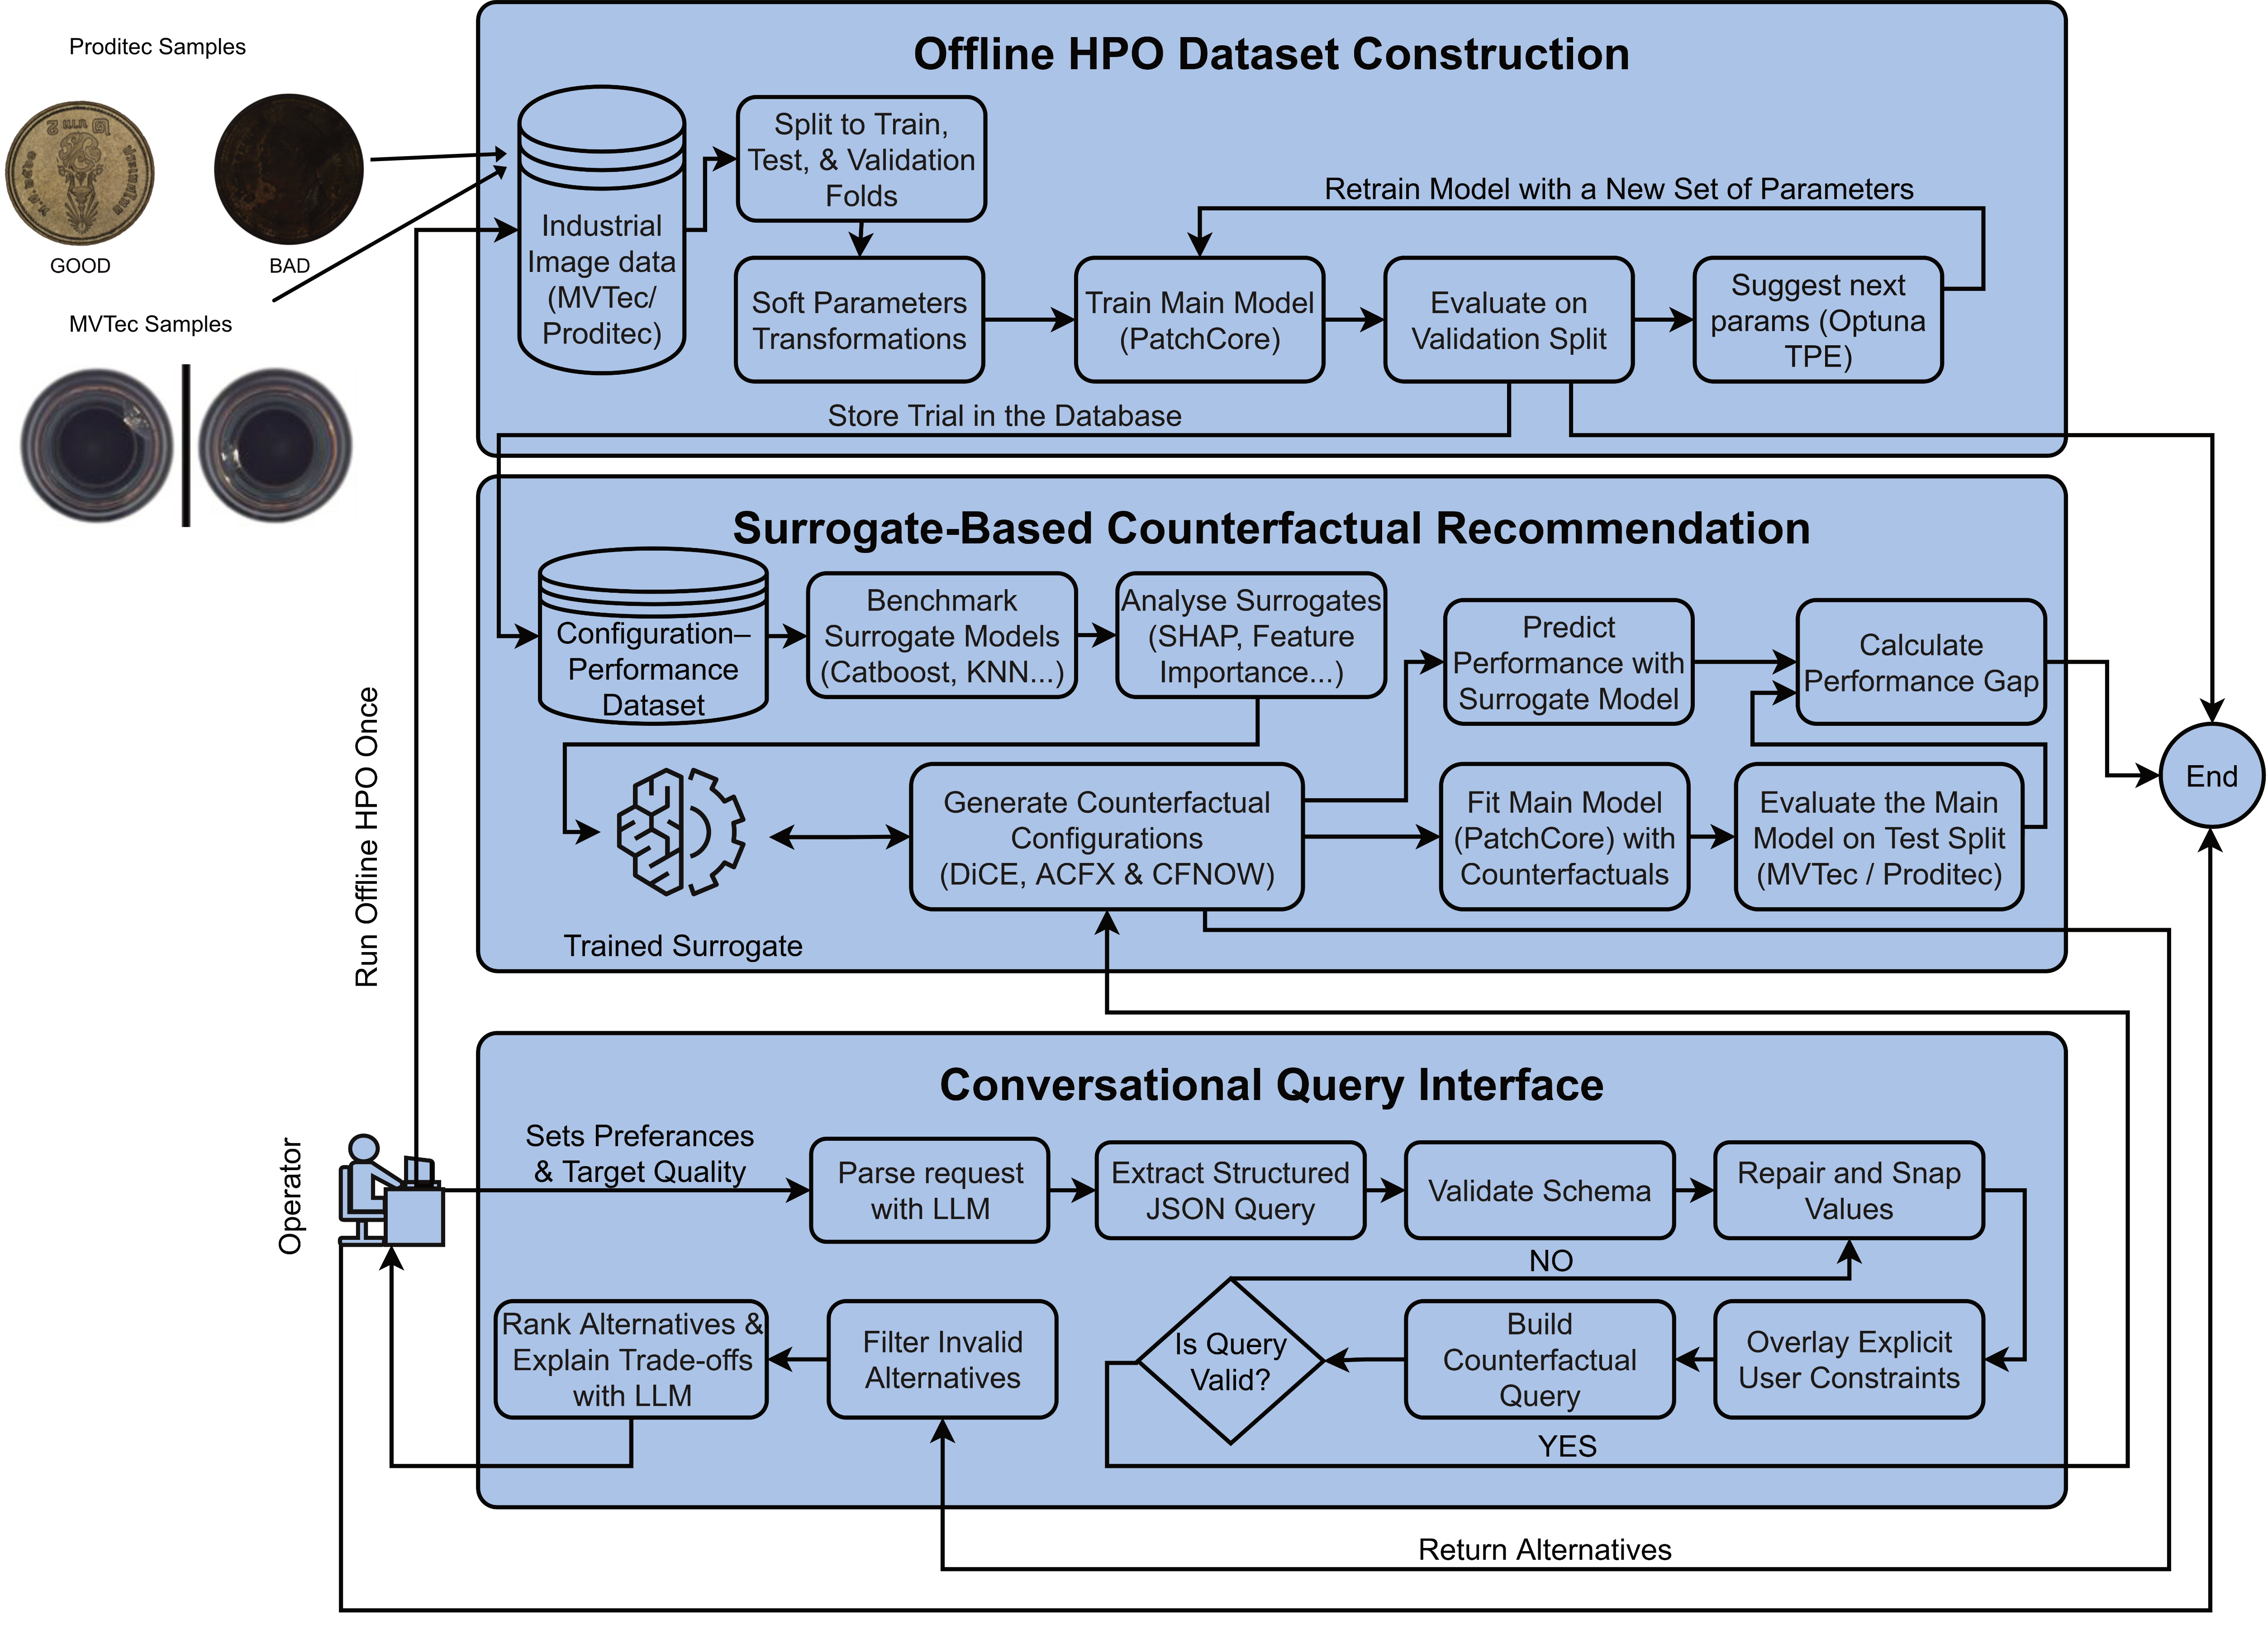
\includegraphics[width=0.64\textwidth]{framework_overview.png}
    \caption{Framework overview. HPO denotes hyperparameter optimisation;
    TPE, tree-structured Parzen estimator; KNN, k-nearest neighbours;
    SHAP, Shapley additive explanations; DiCE, Diverse Counterfactual
    Explanations; ACFX, Actionable Counterfactual Explanations; LLM,
    large language model; and JSON, JavaScript Object Notation. CFNOW
    denotes the archived-code label for \textsc{LogTopK} in this figure,
    not the published CFNOW algorithm.}
    \label{fig:framework-overview}
\end{figure*}

\subsection{Optimisation Logs and Configuration Features}
\label{subsec:logs-features}

Each completed HPO trial produces a record:
\begin{equation}
    (\mathbf{x}_i, v_i) = ((\mathbf{h}_i, \mathbf{s}_i), v_i),
    \label{eq:trial-record}
\end{equation}
where $v_i = v(\mathbf{x}_i)$ is the validation F1 score obtained by
training and evaluating the pipeline under that configuration. Given
$N$ completed trials, the complete optimisation log is:
\begin{equation}
    \mathcal{D}_{\mathrm{log}} = \{(\mathbf{x}_i, v_i)\}_{i=1}^{N}.
    \label{eq:log-dataset}
\end{equation}

In our implementation, hard hyperparameters define the PatchCore-style
pipeline: backbone, batch size, centre crop, coreset ratio, image size,
feature layers, maximum patches per image, nearest neighbours,
pretrained weights, and anomaly-score reduction; the soft controls are
defined in Section~\ref{subsec:problem-formulation}. We deterministically
cast categorical features, snap continuous controls, discard invalid or
incomplete trials, and retain only features used by the surrogate and
candidate-production methods. The cleaned MVTec and Proditec logs
contain $9{,}976$ and $2{,}999$ trials, respectively.

Table~\ref{tab:configuration-space} lists the configuration variables;
the same space applies to both use cases.

\begin{table}[!t]
\centering
\footnotesize
\renewcommand{\arraystretch}{1.0}
\caption{Configuration variables used in the proposed framework (hard
hyperparameters and soft controls). The corruption level is applied by
the experimenter to the training images (Section~\ref{subsec:protocol}).}
\label{tab:configuration-space}
\begin{tabular}{@{}p{0.30\columnwidth}p{0.60\columnwidth}@{}}
\toprule
Variable & Domain / Values \\
\midrule
\multicolumn{2}{@{}l}{\emph{Hard hyperparameters}}\\
Backbone & \texttt{wide\_resnet50\_2}, \texttt{resnet18}, \texttt{resnet34}, \texttt{resnet50} \\
Batch size & \{8, 16\} \\
Centre crop & \{\texttt{none}, \texttt{0.875}\} \\
Coreset ratio & $[0.001, 0.101]$, step $0.002$ \\
Image size & \{224, 256, 320\} \\
Feature layers & \{\texttt{l2}, \texttt{l3}, \texttt{l2\_l3}, \texttt{l1\_l2\_l3}\} \\
Maximum patches/image & \{128, 256, 512, 1024\} \\
Neighbours & $[1, 30]$ \\
Pretrained weights & \{\texttt{True}, \texttt{False}\} \\
Reduction & \{\texttt{max}, \texttt{mean}\} \\
\midrule
\multicolumn{2}{@{}l}{\emph{Soft controls}}\\
Training fraction & $[0.20, 1.00]$, step $0.01$ \\
Review budget & $[0.005, 0.500]$, step $0.005$ \\
Corruption level & \{\texttt{none}, \texttt{mild}, \texttt{strong}\}\\
\bottomrule
\end{tabular}
\end{table}

\subsection{Surrogate-Based Performance Modelling}
\label{subsec:surrogate}

Training the main anomaly-detection model for every possible user
query would be computationally expensive. The framework therefore
trains a surrogate model:
\begin{equation}
    \hat{f}_{\theta}: \mathcal{X} \rightarrow [0,1],
    \label{eq:surrogate}
\end{equation}
where $\mathcal{X}$ is the mixed categorical--numerical configuration
space and $\hat{f}_{\theta}(\mathbf{x})$ is the predicted validation
F1 score. The surrogate is trained on a training split
$\mathcal{D}_{\mathrm{train}} \subseteq \mathcal{D}_{\mathrm{log}}$ (the
exact split used in our experiments is given in
Section~\ref{subsec:protocol}) by minimising the squared prediction
error:
\begin{equation}
    \mathcal{L}(\theta)
    =
    \frac{1}{|\mathcal{D}_{\mathrm{train}}|}
    \sum_{(\mathbf{x}_i,v_i)\in \mathcal{D}_{\mathrm{train}}}
    \left(v_i - \hat{f}_{\theta}(\mathbf{x}_i)\right)^2.
    \label{eq:surrogate-loss}
\end{equation}

The surrogate approximates quality for unseen or modified
configurations and lets candidate-production methods search for
configurations meeting a target without retraining PatchCore.
Generated candidates need not coincide with any logged trial, so for
them the surrogate is the only estimate, and whether generation beyond
the log is \emph{needed} is tested in
Section~\ref{subsec:retrieval-comparison}. The surrogate is a search
layer, not final evidence; selected recommendations are confirmed with
the underlying model.

\subsection{Counterfactual Configuration Generation}
\label{subsec:cf-generation}

Given a factual configuration $\mathbf{x}_0$ and a user query, the
counterfactual generation layer searches for alternative configurations
$\mathbf{x}'$ that meet a desired performance objective while
respecting user-defined constraints. The user objective is converted
into a desired prediction interval $R(q, \mathbf{x}_0) = [L, U]$,
where $q$ denotes the structured query. The framework supports three
objective types:
\begin{equation}
R(q,\mathbf{x}_0)=
\begin{cases}
[v, 1], & \text{if } q_{\mathrm{obj}}=\texttt{target\_min}(v), \\
[\hat{f}_{\theta}(\mathbf{x}_0)+\delta, 1],
        & \text{if } q_{\mathrm{obj}}=\texttt{delta\_improve}(\delta), \\
[L, U], & \text{if } q_{\mathrm{obj}}=\texttt{target\_band}(L,U).
\end{cases}
\label{eq:objective-types}
\end{equation}

Soft constraints restrict the candidate space for operator-facing
controls. For numerical controls such as training fraction and review
budget, a constraint can be free, fixed to a value, or restricted to a
range. For the categorical corruption level, it can be free, fixed, or
restricted to an allowed set. These constraints define a feasible
region:
\begin{equation}
    \mathcal{X}_{q} = \{\mathbf{x} \in \mathcal{X} :
    \mathbf{s} \text{ satisfies the soft constraints in } q\}.
    \label{eq:query-feasible-region}
\end{equation}

A candidate satisfies its recorded query under the surrogate when:
\begin{equation}
    \hat{f}_{\theta}(\mathbf{x}') \in R(q,\mathbf{x}_0),
    \qquad
    \mathbf{x}' \in \mathcal{X}_{q}.
    \label{eq:cf-validity}
\end{equation}
The proportion of candidates satisfying Eq.~\ref{eq:cf-validity} is the
\emph{surrogate-level query satisfaction rate}; the \emph{confirmation
rate} is the proportion whose retrained PatchCore score meets the same
objective (Section~\ref{subsec:cf-validity}). Reporting both prevents
surrogate-level compliance from being mistaken for evidence about the
underlying model. When too few query-satisfying alternatives exist, the
system retains near-compliant candidates, marks unmet constraints, and
ranks them below fully compliant alternatives.

Candidate production compares two generators with one retrieval
method: DiCE \cite{10.1145/3351095.3372850} produces diverse
alternatives; Actionable Counterfactual Explanations (ACFX)
\cite{bobek_acfx} uses explainable boosting machines to seek
alternatives close to the factual; and \textsc{LogTopK} filters logged
trials by the query constraints and re-ranks them with the surrogate,
so it cannot leave the log (the archived notebooks call it
\texttt{CFNOW}, but it is not the CFNOW tabu-search algorithm
\cite{DEOLIVEIRA2023}). Each method receives the factual, the
surrogate, the desired interval, the permitted ranges, and $K$:
\begin{equation}
    \mathcal{C}_{m} =
    G_{m}(\mathbf{x}_0, \hat{f}_{\theta}, R, \mathcal{X}_{q}, K),
    \label{eq:generator}
\end{equation}
where $G_m$ denotes the procedure used by method $m$.

Candidates are post-processed to remove invalid rows, enforce feature
domains, and rank alternatives. Ranking prioritises objective
satisfaction, soft-constraint satisfaction, predicted quality, and
proximity to the factual configuration. Proximity is measured by a
mixed-type distance:
\begin{equation}
    d(\mathbf{x}',\mathbf{x}_0)
    =
    \sum_{j \in \mathcal{N}}
    \frac{|x'_j - x_{0j}|}{r_j}
    +
    \sum_{j \in \mathcal{C}}
    \mathbb{I}[x'_j \neq x_{0j}],
    \label{eq:mixed-distance}
\end{equation}
where $\mathcal{N}$ and $\mathcal{C}$ are the numerical and categorical
feature sets, and $r_j$ is the range of numerical feature $j$.

\subsection{Conversational Query Interface}
\label{subsec:interface}

The conversational interface allows users to express configuration
goals in natural language while keeping the recommendation process
constrained and reproducible. A user request $u$ is mapped to a
structured query $q = \Phi(u)$, where $\Phi$ denotes the
language-model-based parser followed by deterministic validation,
repair, normalisation, and snapping. The parser is implemented with an
instruction-tuned open-weight language model behind a fixed JSON schema.
The deployment used in the user study called
\texttt{qwen/qwen-2.5-7b-instruct} through the OpenRouter API; the
released offline front-end runs Qwen2.5-3B-Instruct locally (Phi-3-mini
and Llama-3.2-3B are supported alternatives), and
Section~\ref{subsec:parser-eval} evaluates both.

The structured query has three components. The \emph{objective} is
\texttt{target\_min}($v$), \texttt{delta\_improve}($\delta$), or
\texttt{target\_band}($L,U$). The \emph{soft constraints} give
training fraction and review budget as \texttt{free},
\texttt{fixed}, or \texttt{range}, and corruption level as
\texttt{free}, \texttt{fixed}, or \texttt{allowed}. The
\emph{selection} request is an integer $K$. For example, \emph{``Find me three configurations with F1 at least 0.85
and review budget below 0.30, training on no more than 60\% of the
data''} maps to \texttt{target\_min(0.85)} with
\texttt{review\_budget: range(0, 0.30)} and
\texttt{training\_fraction: range(0, 0.60)}; \emph{``10\% less review
effort at similar quality''} is representable as
\texttt{delta\_improve(0.0)} with \texttt{review\_budget: range(0,
0.90\,*\,current\_budget)}, but relative requests of this form are not reliably produced by the parser (Section~\ref{subsec:parser-eval}): they may trigger the fallback or yield schema-valid queries with incorrect numerical bounds; deterministic resolution (extract field,
direction, and percentage, compute the bound in code) is not yet
implemented.

The language model must return only JavaScript Object Notation (JSON)
matching the schema; the output is normalised, validated, repaired, and
snapped to valid domains (the review-budget grid, a clipped and
quantised training fraction, the allowed corruption levels), and
explicit numerical preferences in the request are overlaid after
parsing so that user-stated values take precedence over ambiguous
model interpretations.

The factual reference for generation is resolved automatically from
the optimisation log: after scoring all trials with the surrogate, the
interface selects $n$ anchor trials ($n{=}3$ by default) combining the
best-predicted trial, a median-budget trial from the upper predicted
range, and greedily diversity-maximising additions. The validated
query is applied at each anchor; per-anchor candidates are pooled,
deduplicated, ranked by predicted quality, and truncated to the
requested $K$.

The interface presents alternatives in a compact table (predicted
quality, main configuration choices, soft-control values, constraint
status), followed by a textual explanation that summarises the
objective, compares alternatives, identifies best and runner-up,
reports ties, and surfaces shared violations once. In the released
interface this text is rendered by a deterministic template from the
structured payload, so every number in it is copied from the table,
and a fixed note states that the summary is generated automatically and
has not been audited beyond that. The study-time interface additionally
passed the template through the language model for fluency; a post-hoc
numeric audit of those 51 polished explanations is reported in
Section~\ref{subsec:limitations}. The language model is thus confined
to translating intent into a structured query and, in the study, to
rephrasing a structured payload, while ranking, constraint checks, and
candidates remain grounded in the surrogate, the feature domains, and
the candidate-production method.

% =======================================================================
\section{Technical Evaluation}
\label{sec:evaluation}
% =======================================================================

This section evaluates the pipeline on MVTec, the controlled
benchmark, and Proditec, the production use case: surrogate fidelity
(Section~\ref{subsec:surrogate-fidelity}), query satisfaction and
main-model confirmation of 24 candidates per dataset
(Sections~\ref{subsec:cf-validity}--\ref{subsec:gap-diagnosis}), and
the diagnostic analyses of
Sections~\ref{subsec:multi-factual}--\ref{subsec:parser-eval}.

\subsection{Datasets and Use Cases}
\label{subsec:datasets}

\paragraph{MVTec AD}
In our evaluation, MVTec \cite{bergmann_mvtec_2019} provides controlled
train/validation/test splits and a well-understood performance
landscape, serving as the benchmark half of the two-dataset comparison.
Our MVTec configuration log contains $9{,}976$ completed trials over
the PatchCore configuration space across four of the fifteen MVTec
categories (bottle, cable, capsule, hazelnut). This restriction is a compute-budget decision fixed in advance rather
than chosen on downstream results: every logged trial retrains
PatchCore, so four categories alone cost roughly $77$ hours of graphics
processing unit (GPU) time
(Section~\ref{subsec:compute-cost}) and all fifteen would scale that
by about $4\times$.

\paragraph{Proditec}
Proditec is a production dataset from an inline coin-inspection system:
images of several coin denominations captured from fixed camera
positions during one acquisition campaign and labelled good or
defective at image level, without defect-type annotation. Unlike MVTec,
the images reflect production variability, sensor noise, and imbalanced
defect frequencies, which lets us test whether the pipeline generalises
from benchmark to deployment. The images are proprietary; we release
the derived logs, features, and models. The split uses $4{,}538$ normal
training images and $867$ held-out images each for validation ($567$
normal / $300$ defective) and test ($568$ / $299$); images are resized
to the configured input size and optionally centre-cropped
(Table~\ref{tab:configuration-space}). Our Proditec configuration log
contains $2{,}999$ completed trials over the same configuration space.



\subsection{Experimental Protocol}
\label{subsec:protocol}

All experiments ran on a single workstation with one NVIDIA RTX~A5500
GPU (power-capped to 70\% of its board limit), an AMD Threadripper PRO
5995WX central processing unit (CPU), and 256 gigabytes of memory. Optuna logs were collected independently for each use case; invalid or
incomplete trials are removed, categorical variables normalised,
numerical variables snapped to their domains, and the remaining trials
train the surrogate (Eqs.~\ref{eq:surrogate}--\ref{eq:surrogate-loss}).
The original stratified $80/20$ split is retained as a development
comparison only, because CatBoost uses its $20\%$ portion for early
stopping; the primary fidelity estimate is the grouped cross-validation
of Section~\ref{subsec:surrogate-fidelity}.

A CatBoost regressor \cite{prokhorenkova_catboost_2018} is used as the surrogate because it provides
native handling of categorical configuration features and competitive
predictive performance on the configuration--performance dataset. On
each dataset, the surrogate is queried by three candidate-production
methods: DiCE, \textsc{LogTopK}, and ACFX, each instantiating the call of Eq.~\ref{eq:generator}. For each method
we request $K = 8$ candidates, yielding $24$ per dataset. This provides
several alternatives while keeping full confirmation feasible. When
query-satisfying candidates are insufficient, the fallback of
Section~\ref{subsec:cf-generation} retains explicitly marked
near-compliant candidates.
Candidates are filtered and ranked according to objective satisfaction,
soft-constraint satisfaction, predicted quality, and distance from the
factual configuration. A candidate satisfies its surrogate query if it meets
Eq.~\ref{eq:cf-validity} within the feasible region of
Eq.~\ref{eq:query-feasible-region}.
Since the technical evaluation has no live operator, the factual
configuration $\mathbf{x}_0$ is a logged trial chosen by the
experimenter from a pipeline-presented set containing the trials
nearest the 50th, 70th, 85th, and 95th validation-F1 percentiles plus
the best trial. The selected factual is held fixed across all three
methods. On both datasets the selected primary factual is the best
logged trial (MVTec: trial $4523$, validation F1 $0.820$, $99.97$th
percentile of the log; Proditec: trial $2738$, $0.908$, $99.97$th
percentile), chosen before any confirmation was run; Section~\ref{subsec:multi-factual} reports the full anchor sweep. For exact reproduction,
\path{mvtec_all_methods_cfs_metadata.json} and
\path{proditec_all_methods_cfs_metadata.json} record the primary
\texttt{factual\_index}, which resolves the complete feature vector in
the released trial table; all three methods load that same payload.
Both datasets use the same methods, $K$, and free soft controls. The
recorded MVTec objective is \texttt{target\_min(0.70)}; Proditec uses
\texttt{target\_band(0.75,0.95)} (Eq.~\ref{eq:objective-types}).

Finally, every candidate is confirmed with the underlying PatchCore
pipeline under the protocol of the HPO objective
(Eq.~\ref{eq:hpo-target}): on MVTec one model and one
validation-calibrated threshold per category, with the four
per-category F1 scores averaged; on Proditec a single model.
Confirmation recomputes validation and test F1 and test AUROC. All 24
candidates per dataset were retrained under three seeds (42, 43, 44) in
one frozen run, and every confirmation number in this paper is taken
from that run; the \emph{gap} is confirmed test F1 minus surrogate F1
unless stated otherwise. The mean seed-to-seed F1 standard deviation is
$0.009$ on MVTec and $0.004$ on Proditec for pretrained backbones, so
method differences below about $0.02$ are not interpreted.
To check that logged scores reproduce, the same run also retrained 96
logged trials in total (48 per dataset: 40 stratified across the F1
range and the 8 best) under the same three seeds. Pretrained-backbone
trials reproduce their logged validation F1 with a mean absolute
difference of $0.004$ on MVTec and $0.007$ on Proditec (maximum $0.018$; the Proditec maximum of $0.070$ is a low-scoring trial with logged F1 $0.32$), and the eight best MVTec trials re-measure $0.008$ below
their logged value, so the log carries no material winner's curse.
Random-initialisation backbones are unstable (seed standard deviation up
to $0.10$ on Proditec); none of the 48 recommendations uses one.

\paragraph{Implementation details}
PatchCore is our own implementation over torchvision feature
extractors (\texttt{wide\_resnet50\_2}, \texttt{resnet18/34/50}, with
ImageNet weights when \texttt{pretrained} is true) rather than a
packaged library. Corruption is applied deterministically to training
(normal) images only, seeded per image path: \texttt{mild} is a
Gaussian blur of radius $0.6$; \texttt{strong} is a Gaussian blur of
radius $1.2$ followed by additive Gaussian noise ($\sigma = 8$ on the
$0$--$255$ scale, clipped); \texttt{none} leaves images unchanged.
Held-out images are divided into validation and test halves by a label-stratified $50/50$ split, per MVTec category and once for Proditec (anomaly prevalence $0.70$ pooled over the MVTec categories, $0.345$ on Proditec). HPO uses
Optuna's TPE sampler (fixed seed, \texttt{multivariate=False},
\texttt{group=False}), with $1{,}500$ start-up trials for Proditec and
$4{,}000$ for MVTec, maximising
Eq.~\ref{eq:hpo-target}, with no pruning and a fixed trial budget. The
surrogate is CatBoost ($5{,}000$ iterations with early stopping after
$200$ rounds, learning rate $0.05$, depth $8$, \texttt{l2\_leaf\_reg}
$3.0$, root mean squared error loss). DiCE runs in regression mode (\texttt{model\_type="regressor"},
\texttt{method="random"}) with the desired range $R(q,\mathbf{x}_0)$ of
Eq.~\ref{eq:objective-types} as target interval, per-feature ranges
taken from the observed log domain, and a raw pool of $\max(30, 10K)$
candidates before repair. ACFX requires a binary target: every logged
configuration is labelled $1$ if its CatBoost-predicted F1 lies in
$R(q,\mathbf{x}_0)$ and $0$ otherwise, a main-effects explainable
boosting machine classifier (\texttt{interpret},
\texttt{interactions=0}) is fitted to these labels, and ACFX
counterfactuals towards class $1$ are generated around the factual. All
final candidates are rescored with the common CatBoost surrogate, so the
three methods share final scoring.
Software: Python 3.11.9,
PyTorch 2.10.0 (CUDA 12.8), torchvision 0.25.0, scikit-learn 1.6.1,
Optuna 4.2.0, CatBoost 1.2.8, dice-ml 0.12, acfx 0.3.6, interpret
0.7.3, transformers 5.1.0.

\subsection{Surrogate Fidelity}
\label{subsec:surrogate-fidelity}

We benchmarked $13$ candidate regressors for the surrogate role
(twelve scikit-learn \cite{pedregosa_scikit-learn_2011} models plus CatBoost);
the two most relevant are CatBoost, the operational surrogate, and HistGradientBoosting, the strongest alternative, which are indistinguishable on the development split (RMSE $0.015$ / $0.086$, MAE $0.008$ / $0.046$, $R^2$ $0.996$ / $0.936$ for CatBoost on MVTec / Proditec; $0.015$ / $0.085$, $0.008$ / $0.043$, $0.996$ / $0.937$ for HistGradientBoosting). We selected CatBoost not
because it topped the benchmark but because it handles the mixed
categorical--numerical space natively for the downstream
counterfactual pipeline and ships built-in feature-importance and
Shapley tooling, so the surrogate's behaviour is directly inspectable
as required by the paper's interpretability focus. As a robustness
check we also trained a Gaussian process (GP) surrogate on a 1,500-trial
subsample; it achieves $R^2 = 0.990$ and $R^2 = 0.919$ on MVTec and
Proditec respectively with well-calibrated uncertainty (90\% prediction
interval coverage $0.89$ and $0.90$), confirming that the high fidelity
is not specific to CatBoost. We retain CatBoost for the deployed system
because of its native categorical handling and faster inference; the
GP's calibrated intervals are the natural basis for the per-candidate
support indicator the system still lacks (Section~\ref{subsec:limitations}).





The two surrogates differ in error profile: development-split RMSE is $0.015$ on MVTec and $0.086$ on Proditec, over validation-F1 ranges of roughly $0.02$--$0.82$ and $0.0$--$0.91$. To understand where each surrogate's predictive power comes from, we ablated the model and computed SHAP importances.
On MVTec the review-budget feature alone accounts for $75.3\%$ of the
full-model SHAP magnitude, and removing it collapses $R^2$ from $0.995$ to $0.098$ (Table~\ref{tab:surrogate-ablation}); the
remaining hard hyperparameters carry the rest. On Proditec the budget
share is lower ($23.0\%$), and the top SHAP features are the feature
layer choice ($21.8\%$) and pretrained weights ($14.1\%$), reflecting
that the production use case involves both architecture choices and
operational trade-offs in its optimisation target; removing the review budget reduces $R^2$ to $0.749$. This asymmetry cautions
against treating cross-dataset $R^2$ comparisons as equivalent: the
MVTec surrogate is largely a monotone review-budget function, while
Proditec's involves genuine hyperparameter structure.

To confirm that fidelity holds across the query-relevant score range
and not only in aggregate, we computed $R^2$ within each review-budget
band (five equal-count bands of the logged budget values; 381--415 trials per band on MVTec, 112--132 on Proditec). From the lowest to the highest band, $R^2$ is $0.986$, $0.966$, $0.923$, $0.914$, and $0.938$ on MVTec (median $0.938$) and $0.876$, $0.846$, $0.936$, $0.879$, and $0.910$ on Proditec (median $0.879$), so the surrogate is locally consistent
in the query-relevant regions used to generate candidates. Nor is it
optimistic where a query selects: binned by predicted quantile, the
mean signed error of predicted minus recorded F1 is within $\pm 0.001$
on MVTec and within $\pm 0.007$ on Proditec for the top $10\%$ of
predictions, so the surrogate does not inherit a winner's curse from
the log.

To complement absolute error reporting, we also compute scale-normalised
metrics: relative RMSE (rRMSE, normalised by the mean~\cite{jin2024officegpr}) is $2.9\%$ on MVTec and $17.0\%$ on Proditec. The difference between the two surrogates is consistent with the ablation above rather than with the range of the target: the MVTec objective is largely a function of the review budget, which the surrogate recovers almost exactly, whereas the Proditec objective depends on hard hyperparameters whose effect is harder to predict.

\begin{table}[!t]
\centering
\footnotesize
\caption{Surrogate ablation: development-split $R^2$ of CatBoost models
re-trained on feature subsets with inner early stopping (MVTec and
Proditec). ``Budget only'' uses the review budget as the single feature;
``hard HPs only'' removes all soft controls. Because of the inner
early-stopping split, the full-model row differs slightly from the development-split value (0.936) and from the grouped estimate (0.934).}
\label{tab:surrogate-ablation}
\setlength{\tabcolsep}{3pt}
\begin{tabular}{@{}lrr@{}}
\toprule
Feature set & MVTec $R^2$ & Proditec $R^2$ \\
\midrule
Full model (13 features)    & 0.995 & 0.944 \\
Without review budget       & 0.098 & 0.749 \\
Review budget only          & 0.963 & 0.477 \\
Hard hyperparameters only   & 0.086 & 0.753 \\
\bottomrule
\end{tabular}
\end{table}

Because TPE revisits promising regions, the logs contain exact
duplicate configurations ($15.0\%$ of MVTec rows, $17.6\%$ of
Proditec rows), and a shuffled split places $19.9\%$ and $26.2\%$ of
test configurations next to an identical training row. The primary
generalisation estimate is therefore 5-fold GroupKFold cross-validation
grouped by configuration signature with fixed 500-iteration models:
$R^2 = 0.995 \pm 0.0005$ on MVTec and $0.934 \pm 0.008$ on Proditec,
matching the development values, so the fidelity conclusion is not an
artefact of duplicate leakage. 

\subsection{Surrogate Query Satisfaction and Main-Model Confirmation}
\label{subsec:cf-validity}

Surrogate-level query satisfaction is 24/24 on both datasets: every
candidate meets its recorded objective and soft constraints under
Eq.~\ref{eq:cf-validity}. Main-model confirmation under the protocol of
the HPO objective gives the same count: all 24 Proditec candidates fall
inside the requested $[0.75, 0.95]$ band (minimum three-seed mean
$0.814$) and all 24 MVTec candidates exceed the $0.70$ minimum (minimum
$0.758$). The first figure verifies the structured search and constraint layer;
the second shows that the surrogate estimate persists in PatchCore. The
second count has limited discriminating power, however: $29\%$ of all
$9{,}976$ MVTec trials and every trial in the top decile of the log
(validation F1 $0.803$--$0.820$) already exceed $0.70$, and $43\%$ of
Proditec trials and the whole top decile ($0.895$--$0.908$) already lie
in the $[0.75, 0.95]$ band, so meeting the target mostly shows that the
candidates stay near the top of the log.
Section~\ref{subsec:gap-diagnosis} compares the pooled and per-category
protocols and adds an untuned reference.

\subsection{Comparison of Candidate-Production Methods}
\label{subsec:cf-comparison}

Under the primary factual configuration,
Table~\ref{tab:technical-evaluation-summary} summarises generation and
confirmation for both datasets. Two observations stand out. First, all
three methods deliver confirmed F1 above target on both datasets
(MVTec $0.781$--$0.793$, Proditec $0.863$--$0.889$), with gaps of
$-0.016$ to $-0.034$ on MVTec and $-0.001$ to $-0.011$ on Proditec.
Second, proximity and runtime differ between methods. At the primary
anchor ACFX is closest to the factual on MVTec ($0.13$) and DiCE on
Proditec ($0.10$); DiCE is fastest ($0.3$--$0.5$\,s per eight-candidate call), \textsc{LogTopK} takes a few seconds because the archived implementation re-scores the filtered log on every query, and ACFX is two orders of magnitude slower ($100$--$117$\,s per call). Because the two
datasets use different objectives, their confirmed-F1 levels are not
comparable across the horizontal rule.

Confirmed PatchCore F1 is stable within methods: across-candidate
standard deviations are $0.010$--$0.015$ on MVTec and $0.005$--$0.028$
on Proditec, against three-seed standard deviations of $0.009$ and
$0.004$. The largest difference between method means on MVTec
($0.012$) is within this noise, so we do not rank the methods by
confirmed quality. Complete per-candidate results are included in the
public archive.

\begin{table*}[!tb] \centering \footnotesize \caption{Candidate-production and confirmation results at the primary
anchor (eight candidates per method; PatchCore test F1 as
mean\,$\pm$\,standard deviation \emph{across candidates} of the
three-seed means, not across seeds). Surrogate-level query satisfaction
was 100\% in all six cells. Gap = PatchCore F1 minus surrogate F1.
Distance is the mixed-type measure of Eq.~\ref{eq:mixed-distance}
summed over the 13 configuration features
(Section~\ref{subsec:multi-factual} gives the anchor sweep). Time is the wall-clock generation time of the eight-candidate call (s). MVTec uses the per-category protocol; AUROC is the mean per-category test AUROC on MVTec and the
test AUROC on Proditec. The two datasets used different objectives;
figures are not comparable across the horizontal rule. The archived
code labels \textsc{LogTopK} as \texttt{CFNOW}
(Section~\ref{subsec:cf-generation}).}
\label{tab:technical-evaluation-summary}
\setlength{\tabcolsep}{4.5pt}
\begin{tabular}{@{}lllrrrrrr@{}}
\toprule
Dataset & Method & Objective & Distance & Time & Surrogate &
PatchCore & Gap & AUROC \\
        &        &           &          & (s)  & F1        &
F1        &     &       \\
\midrule
MVTec    & ACFX             & minimum 0.70 & 0.13 & 117.0 & 0.802 & $0.786 \pm 0.010$ & $-0.016$ & 0.901 \\
MVTec    & \textsc{LogTopK} & minimum 0.70 & 1.41 &   5.6 & 0.815 & $0.781 \pm 0.015$ & $-0.034$ & 0.915 \\
MVTec    & DiCE             & minimum 0.70 & 0.77 &   0.3 & 0.813 & $0.793 \pm 0.011$ & $-0.021$ & 0.922 \\
\midrule
Proditec & ACFX             & band 0.75--0.95 & 0.28 & 99.9 & 0.870 & $0.863 \pm 0.028$ & $-0.007$ & 0.976 \\
Proditec & \textsc{LogTopK} & band 0.75--0.95 & 0.22 &  1.4 & 0.897 & $0.886 \pm 0.005$ & $-0.011$ & 0.975 \\
Proditec & DiCE             & band 0.75--0.95 & 0.10 &  0.5 & 0.890 & $0.889 \pm 0.005$ & $-0.001$ & 0.977 \\
\bottomrule
\end{tabular}
\end{table*}

\subsection{Main-Model Confirmation}
\label{subsec:main-model-confirmation}

The central technical result is that main-model confirmation agrees with the surrogate on both datasets once the confirmation protocol matches the optimisation objective. On Proditec, the 24
recommendations average confirmed test F1 of $0.879$, a gap of
$-0.007$, and test AUROC of $0.976$; all 24 fall in the requested band.
On MVTec under the per-category protocol, mean confirmed F1 is $0.787$
(gap $-0.023$), the re-measured validation F1 equals the surrogate
prediction to three decimals ($0.810$), per-category test AUROC is
$0.913$, and all 24 exceed the $0.70$ minimum. Applying one pooled threshold to the concatenated scores of the same 24 per-category models gives $0.570$ (gap $-0.240$), a different quantity (Section~\ref{subsec:gap-diagnosis}). Main-model confirmation remains the final deployment gate in both settings; on these data it confirms the surrogate rather than contradicting it.

Figure~\ref{fig:surrogate-vs-test} plots confirmed against surrogate
F1 for all 48 candidates with seed error bars. On Proditec the points
follow the identity line (Spearman $0.58$), with the two largest gaps
among ACFX candidates at review budget $0.455$. On MVTec the confirmed
scores lie $0.02$--$0.03$ below the surrogate and are not ordered by it
(Spearman $-0.20$ against test F1, $0.80$ against validation F1): the
surrogate predicts its own target almost exactly (mean error $+0.000$),
and the residual is the validation-to-test shift of the threshold,
which is as large as the spread between candidates ($0.012$).

\begin{figure*}[!tb]
\centering
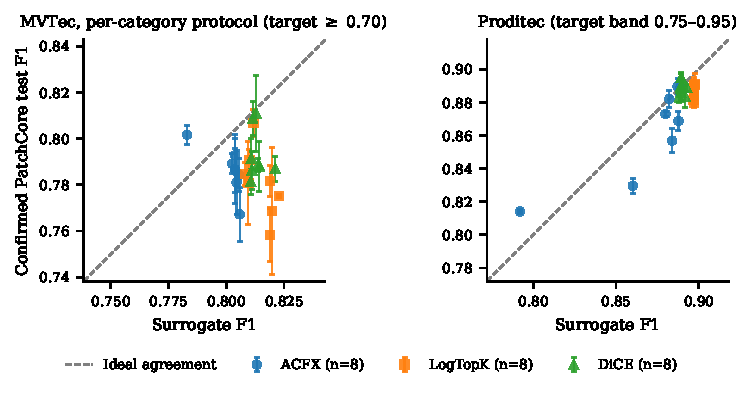
\includegraphics[width=0.8\textwidth]{fig_surrogate_vs_confirmed_both.pdf}
\caption{Confirmed PatchCore test F1 (mean of three seeds; error bars
show the seed standard deviation) against surrogate F1 for the 24 MVTec
candidates under the per-category protocol (left) and the 24 Proditec
candidates (right); the query targets ($0.70$ and $0.75$) lie below both axis ranges.}
\label{fig:surrogate-vs-test}
\end{figure*}

The 48 recommendations are local to a strong anchor. All 24 Proditec
candidates share the best trial's backbone, feature layer, and
clean-data setting (\texttt{resnet34}, \texttt{l3}, no corruption) and
vary in training fraction ($0.68$--$0.97$), review budget
($0.340$--$0.455$), coreset ratio, and neighbours; the six candidates
with the highest confirmed F1 ($0.892$ versus $0.875$ for the other 18)
differ from the rest mainly by a lower review budget ($0.348$ versus
$0.370$; Spearman $-0.39$ between budget and confirmed F1 over the 24).
On MVTec, 23 of 24 candidates use clean training data and all use
pretrained \texttt{wide\_resnet50\_2} or \texttt{resnet50} backbones,
with review budgets at the top of the grid ($0.495$--$0.500$). With 24 non-independent local candidates we report descriptive statistics only.
The primary query therefore tests local fidelity around the best trial;
Section~\ref{subsec:multi-factual} covers weaker anchors.



\subsection{Diagnosing the Confirmation Gap}
\label{subsec:gap-diagnosis}

To understand why the pooled and per-category protocols diverge, we
evaluated the same 24 retrained per-category MVTec models under both thresholding protocols (per-category thresholds, and one pooled threshold over their concatenated scores),
retrained the logged HPO optimum and a no-HPO reference configuration,
and computed the F1 bounds implied by the review-budget rule
(Tables~\ref{tab:gap-diagnosis} and~\ref{tab:per-category}).

\begin{table}[!t] \centering \footnotesize \caption{Protocol diagnosis (means over the 24 confirmed candidates per
dataset). Per-category rows use the three-seed run; the pooled rows apply, for reference, one pooled review-budget threshold to the concatenated scores of the same seed-42 per-category models, so the protocol effect isolates pooled thresholding on identical models. Gap = confirmed test F1 minus surrogate F1. Per-category AUROC is the mean of four per-category
values.}
\label{tab:gap-diagnosis}
\setlength{\tabcolsep}{2.5pt}
\begin{tabular}{@{}p{0.66\columnwidth}rr@{}}
\toprule
Quantity (mean over 24 candidates) & MVTec & Proditec \\
\midrule
Surrogate-predicted F1                                 & 0.810 & 0.886 \\
Re-measured validation F1 (per-category)               & 0.810 & 0.891 \\
Confirmed test F1 (per-category protocol)              & 0.787 & 0.879 \\
Gap (per-category protocol)                            & $-0.023$ & $-0.007$ \\
Confirmed test F1 (per-category protocol, seed-42 models) & 0.785 & -- \\
Confirmed test F1 (pooled protocol, for reference, seed 42) & 0.570 & -- \\
Gap (pooled protocol)                                  & $-0.240$ & -- \\
Protocol effect, same seed-42 models (pooled $-$ per-category) & $-0.215$ & -- \\
\midrule
Per-category test AUROC                                & 0.913 & 0.976 \\
Pooled test AUROC                                      & 0.527 & -- \\
\bottomrule
\end{tabular}
\end{table}

\paragraph{Pooled confirmation measures a different quantity}
The HPO objective (Eq.~\ref{eq:hpo-target}) trains one PatchCore model
per category and computes one review-budget threshold per category.
Applying one pooled threshold to the concatenated scores of the same 24 per-category models yields a score $0.215$ lower ($0.570$ against
$0.785$ for the seed-42 models), although the surrogate error on its own
target is $0.000$ and the validation-to-test shift is $-0.025$: almost
all of the apparent gap under a pooled protocol is the protocol itself,
not the surrogate. Under the per-category protocol all 24 candidates
meet the $0.70$ minimum.

\paragraph{Pooled score-scale incompatibility remains a deployment constraint}
The pooling pathology is still relevant for any deployment that applies
one score threshold across heterogeneous product types. Because
anomaly-score scales differ across categories, merging them destroys
the \emph{global ranking}: the AUROC of the concatenated test scores of the four per-category models is $0.527$, against a mean within-category AUROC of $0.913$ for the same models and scores (Figure~\ref{fig:pooled-vs-perclass}), a ranking-level effect that is independent of any threshold. Applying the review budget within each
category recovers $+0.215$ mean F1 without changing the models.
Operators deploying over several product categories must therefore
calibrate thresholds per category.

\begin{figure}[!t]
\centering
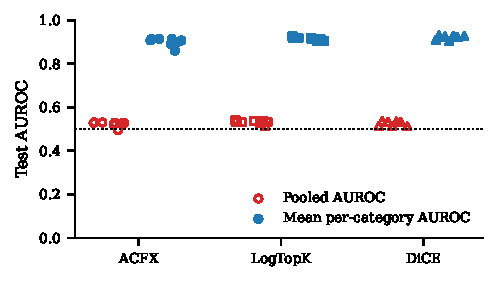
\includegraphics[width=\linewidth]{fig_mvtec_pooled_vs_percategory_auroc.pdf}
\caption{Pooled versus mean per-category test AUROC for each of the 24
confirmed MVTec candidates (seed 42), grouped by method; both values are computed from the same four per-category models, the pooled one on their concatenated scores. Within each category the retrained models rank anomalies well; pooling categories
whose score scales are not commensurable drives the global ranking to
chance.}
\label{fig:pooled-vs-perclass}
\end{figure}

\begin{table}[!t]
\centering
\footnotesize
\caption{Per-category MVTec results at the HPO review budget
($\beta = 0.495$, seed 42): test anomaly prevalence, mean confirmed
test F1 of the 24 candidates, and test F1 / AUROC of the retrained HPO
optimum and of the no-HPO reference configuration. Published PatchCore
image-level AUROC \cite{roth_towards_2022} is given for orientation
only: it uses the official test set without a held-out validation half
and an unsubsampled memory bank.}
\label{tab:per-category}
\setlength{\tabcolsep}{3pt}
\begin{tabular}{@{}lrrrrrrr@{}}
\toprule
 & & Cand. & \multicolumn{2}{c}{HPO optimum} & \multicolumn{2}{c}{Reference} & Publ. \\
Category & Prev. & F1 & F1 & AUROC & F1 & AUROC & AUROC \\
\midrule
bottle   & 0.76 & 0.847 & 0.857 & 0.953 & 0.857 & 0.981 & 1.00 \\
cable    & 0.61 & 0.778 & 0.741 & 0.855 & 0.874 & 0.905 & 0.99 \\
capsule  & 0.82 & 0.624 & 0.659 & 0.864 & 0.813 & 0.968 & 0.98 \\
hazelnut & 0.64 & 0.891 & 0.889 & 0.964 & 0.925 & 0.986 & 1.00 \\
\midrule
mean     & 0.70 & 0.785 & 0.786 & 0.909 & 0.867 & 0.960 & 0.99 \\
\bottomrule
\end{tabular}
\end{table}

\paragraph{No-HPO reference at equal budget}
To test whether the search itself added value, we retrained a reference
configuration without HPO (pretrained \texttt{wide\_resnet50\_2},
layers \texttt{l2\_l3}, input $256$ with centre crop $0.875$, coreset
ratio $0.101$, one neighbour, max reduction, $1{,}024$ patches per
image, full training set, no corruption) on the four categories at the
HPO budget $\beta = 0.495$. The reference reaches test F1 $0.867$ and
AUROC $0.960$, against $0.786$ and $0.909$ for the retrained HPO optimum
(logged $0.820$, re-measured validation $0.809$) and $0.787$ for the mean recommendation (Table~\ref{tab:per-category}); it is better at every budget from $0.2$ to $0.7$ (by $0.03$--$0.09$), and the HPO optimum is better only at $\beta = 0.1$ (by $0.04$). On the HPO objective itself the two
are indistinguishable: validation F1 is $0.812$ for the reference and
$0.809$ for the optimum, and the top tenth of the log (roughly a
thousand trials) lies within $0.80$--$0.82$. The search converged on a
plateau of the validation objective that the objective cannot resolve,
and the test difference reflects which point of that plateau
generalises. In this run (one seed for the optimum and for the reference) and on these four categories, HPO did not improve on the untuned reference configuration, and the recommendations, which inherit the
plateau through the surrogate, do not either; capsule is the weakest
category (candidate F1 $0.624$ against $0.813$ for the reference). Our AUROC is below published PatchCore values because the memory bank is subsampled to at most $1{,}024$ patches per image, half of the official test images are held out for validation, and no ensemble is used; the reference configuration comes within $0.01$--$0.02$ of them on bottle, capsule, and hazelnut, but $0.09$ below on cable ($0.905$ against $0.99$), a gap we have not decomposed and for which no run with an unrestricted memory bank exists.

\paragraph{F1 is bounded by the review-budget rule}
On validation exactly $m_{\beta}$ images are reviewed, so F1 is bounded
for any ranker: with pooled anomaly prevalence $p = 0.70$ and
$\beta = 0.495$, a perfect ranker reaches $2\beta/(\beta+p) = 0.827$
and a random ranker $2\beta p/(\beta+p) = 0.580$; the first is a hard ceiling, the second a reference point, since an anti-correlated ranker scores lower. The HPO optimum
($0.809$) and the reference ($0.812$) both sit near this ceiling, and
the top of the log selects $\beta$ at the top of its grid because F1
under this rule increases with $\beta$ up to the prevalence, which is
why the review budget carries $75\%$ of the surrogate's SHAP mass on
MVTec (Section~\ref{subsec:surrogate-fidelity}). Test F1 is not bounded
in the same way because the validation-calibrated threshold flags a
free number of test images, which is how the reference's test F1
($0.867$) exceeds the validation ceiling. Two consequences follow. The
$0.70$ target lies roughly midway between random and perfect ranking
and is a modest target. And MVTec and Proditec F1 are not comparable at face value: re-weighting the MVTec test positives and negatives to Proditec's prevalence ($0.345$) at the fixed validation-calibrated threshold, the HPO optimum scores $0.752$ and the reference $0.845$. Threshold-free AUROC and
prevalence-matched F1 should accompany review-budget F1 whenever
datasets are compared.

\paragraph{Consequence: the MVTec objective is degenerate at the HPO budget}
F1 runs from $0.58$ for a random ranker to a ceiling of $0.83$, the top tenth of the log lies within
$0.80$--$0.82$, $R^2$ collapses to $0.098$ without the review budget,
all 24 candidates sit at $\beta = 0.495$--$0.500$, and the reference
beats the candidate mean in every category
(Table~\ref{tab:per-category}). MVTec therefore supports the protocol
and objective lessons of this section, not a claim of recommendation
value: the surrogate is reliable on the subset a query selects, while
the objective itself limits what any recommendation can achieve. The
design rules that follow are to match the confirmation protocol to the
HPO objective, to report AUROC and prevalence-matched F1 next to
review-budget F1, to compare against an untuned reference and the
in-band share of the log before attributing value to HPO, to confirm
final candidates with the underlying model, and to calibrate
review-budget thresholds per category for heterogeneous product types.

\subsection{Sensitivity to the Factual Configuration}
\label{subsec:multi-factual}

The main method comparison uses one factual configuration per dataset:
the primary anchor, which is the best logged trial on both datasets
(Section~\ref{subsec:protocol}). As an anchor-sensitivity analysis we
repeated generation under a common target-band query
(\texttt{target\_band} $[0.75,0.95]$, free soft controls, $K=8$) at
five factual anchors spanning the log (the trials nearest the 50th,
70th, 85th, and 95th percentiles of validation F1, plus the best trial)
for the two fast methods, DiCE and \textsc{LogTopK}; ACFX was excluded
because of its generation cost. For every anchor--method cell the three
top-ranked candidates, i.e.\ those an operator would be shown first,
were retrained ($60$ retrainings, seed 42, per-category protocol on
MVTec), and a candidate is verified when its confirmed test F1 meets
the query minimum of $0.75$.

Surrogate-level query satisfaction is $100\%$ in every cell. On
Proditec all $30$ candidates are verified; on MVTec $12/15$
\textsc{LogTopK} and $13/15$ DiCE candidates are, with per-anchor
counts (p50, p70, p85, p95, best) of $2, 3, 2, 2, 3$ and $2, 2, 3, 3,
3$ of $3$. All five failures are marginal ($0.728$--$0.749$ against
$0.75$), all $60$ candidates verify on validation F1, and verification
does not track the anchor (Spearman correlation between anchor
percentile and validation error $0.48$ on MVTec, $0.00$ on Proditec,
$n = 30$). One caveat: \textsc{LogTopK} returns the same top-scoring
logged configurations at every anchor (constant surrogate F1 $0.820$
and $0.898$), so its $15$ cells per dataset are five seeded
replications of three configurations rather than fifteen independent
candidates, and only its distance to the factual varies with the anchor
($1.41$ at the best trial to about $6$ at the median trial on MVTec;
$0.22$ to $3.9$ on Proditec). DiCE adapts to the anchor, trading a
lower surrogate score near weak anchors ($\bar{F}_1$ $0.787$--$0.815$
and $0.858$--$0.895$) for smaller distances near strong ones (down to
$0.43$ and $0.01$).

\subsection{Generation versus Log Retrieval under Constrained Queries}
\label{subsec:retrieval-comparison}

We tested generation beyond the log with twelve structured queries
(broad, tight, absolute, quantile, one-sided, relative, combined, and
infeasible constraints) at three factual anchors per dataset, comparing
DiCE with \textsc{LogTopK} (query-satisfying logged configurations
ranked by surrogate score), \textsc{NearestFeasible} (ranked by the
distance of Eq.~\ref{eq:mixed-distance}), and \textsc{RecordedTopK}, a
filter-and-sort baseline that ranks by \emph{recorded} F1 and does not
use the surrogate at all. For DiCE we report raw counts before repair
and domain snapping as well as final query satisfaction.

Three findings summarise the suite. First, in every query cell where
any method produced query-satisfying candidates, the retrieval
baselines did as well, and DiCE satisfied no query that retrieval could
not; conversely, the absolute tight band $[0.85, 0.90]$, the relative
budget-reduction query, and the combined tight query were infeasible on
MVTec for \emph{all} methods, generation included, because the surrogate
assigns no configuration a score in the requested region ($13$ of $36$
query--anchor cells are answerable on MVTec, $22$ on Proditec). Second,
\textsc{RecordedTopK} answers the same cells as \textsc{LogTopK} and
returns sets of comparable recorded quality: the mean Jaccard overlap
between the two methods' returned sets is $0.26$ on MVTec and $0.15$ on
Proditec, and the mean recorded F1 of the returned sets differs by
$-0.003$ and $+0.002$, so surrogate ranking neither helps nor hurts
retrieval when the log is dense. Third, main-model confirmation of the
top candidates under the tight quantile band (two per method per
dataset, twelve retrainings, per-category protocol on MVTec) shows retrieval no worse than generation in confirmed quality; all differences in Table~\ref{tab:retrieval-confirmed} are below the $0.02$ noise floor.

Across this suite, off-log generation does not increase feasible-query
coverage, and surrogate-ranked, recorded-F1-ranked, and distance-ranked
retrieval give comparable top-candidate quality. For these two logs, retrieval is therefore the appropriate first-stage policy, and because \textsc{RecordedTopK} performs like \textsc{LogTopK}, the surrogate is not needed for retrieval on dense logs; it matters for generation and for scoring configurations outside the log. Because logged status did not guarantee confirmation under every query, retrieval reduces unsupported search but does not replace main-model confirmation.

\begin{table}[!t]
\centering
\footnotesize
\caption{Confirmed generation-versus-retrieval comparison under the
tight quantile band (top two candidates per method at the p85 anchor;
seed 42; per-category protocol on MVTec; means of surrogate and
confirmed PatchCore test F1, their gap, and test AUROC).}
\label{tab:retrieval-confirmed}
\setlength{\tabcolsep}{2pt}
\begin{tabular}{@{}lp{0.22\columnwidth}rrrr@{}}
\toprule
Dataset & Method & Surrogate F1 & Confirmed F1 & Gap & AUROC \\
\midrule
MVTec    & DiCE            & 0.802 & 0.771 & $-0.030$ & 0.919 \\
MVTec    & \textsc{LogTopK}         & 0.808 & 0.789 & $-0.020$ & 0.922 \\
MVTec    & \textsc{Nearest\-Feasible} & 0.800 & 0.773 & $-0.027$ & 0.901 \\
\midrule
Proditec & DiCE            & 0.896 & 0.871 & $-0.025$ & 0.969 \\
Proditec & \textsc{LogTopK}         & 0.898 & 0.890 & $-0.007$ & 0.977 \\
Proditec & \textsc{Nearest\-Feasible} & 0.891 & 0.883 & $-0.008$ & 0.975 \\
\bottomrule
\end{tabular}
\end{table}

\paragraph{Coverage as a function of log density}
We subsampled each log to $50$, $25$, $10$, and $5\%$ of its trials
(three draws each; spread given as the standard deviation across
draws). \textsc{LogTopK} returns a full set of eight candidates for all
answerable MVTec cells down to $25\%$ of the log and for $0.77$ of them
at $10$ and $5\%$ (no spread); on Proditec the share is $0.86$ from
$100$ down to $10\%$ and $0.77 \pm 0.08$ at $5\%$. At least one
candidate is returned for every answerable MVTec cell down to $10\%$
($0.92 \pm 0.13$ at $5\%$) and for $86$--$91\%$ of Proditec cells at
every reduced density; \textsc{RecordedTopK} behaves the same within
$0.05$. DiCE's full-set share does not degrade with density but is
lower on Proditec throughout ($0.61$--$0.68$); on MVTec it is
$0.79$--$0.90$ (spread up to $0.12$) and exceeds retrieval's only at
$10\%$ and below. Operationally, full eight-candidate coverage needs
about a quarter of the MVTec log ($\approx 2{,}500$ trials) and a tenth
of the Proditec log ($\approx 300$ trials); below that retrieval returns
partial sets, and generation is a useful fallback on MVTec but not on
Proditec.

\subsection{Computational Cost and Reuse}
\label{subsec:compute-cost}

We distinguish the cost of one surrogate prediction from the complete
interaction. Table~\ref{tab:compute-cost} compares mean PatchCore
retraining time per candidate in the frozen confirmation run (four
per-category models per MVTec candidate), surrogate latency over 200
warmed-up single-row queries, the retrieval step of \textsc{LogTopK}
and \textsc{RecordedTopK} on cached scores, and the complete
interaction including parsing, candidate production, and explanation.
The interaction range sums measured parse, anchor-scoring, generation,
ranking, and explanation times per method; the two language-model
stages were timed over the 40 labelled utterances of
Section~\ref{subsec:parser-eval} with the local 3B model, once on CPU and once on a GPU in bf16. No
power telemetry was collected, so energy and CO$_2$ estimates are not
reported.

\begin{table}[!t]
\centering
\footnotesize
\caption{Component and complete-interaction wall-clock costs.
Retraining times are per candidate from the frozen three-seed
confirmation run; derived rows use the measured means. ``Break-even
$K$'' is the number of alternatives at which one interaction costs as
much as $K$ sequential retrainings (retrieval or DiCE $\mid$ ACFX). LM
denotes the language model.}
\label{tab:compute-cost}
\setlength{\tabcolsep}{2pt}
\begin{tabular}{@{}p{0.56\columnwidth}rr@{}}
\toprule
Quantity & MVTec & Proditec \\
\midrule
PatchCore retraining per candidate (s)         & 57.8  & 46.5 \\
Surrogate prediction (ms)                      & 2.15  & 2.05 \\
Retrieval step, LogTopK / RecordedTopK (ms)    & 1.4   & 1.4 \\
Sequential eight retrainings (s)               & 462   & 372 \\
Eight-candidate interaction, CPU LM (s)        & 141--258 & 141--241 \\
Eight-candidate interaction, GPU LM (s)        & 6.6--124 & 6.6--107 \\
Interaction + one confirmation, CPU LM (s)     & 199--316 & 188--288 \\
Break-even $K$, CPU LM                         & 2.4 $\mid$ 4.5 & 3.0 $\mid$ 5.2 \\
Break-even $K$, GPU LM                         & 0.11 $\mid$ 2.1 & 0.14 $\mid$ 2.3 \\
\bottomrule
\end{tabular}
\end{table}

The surrogate and retrieval components are four orders of magnitude
faster than one retraining, but with a CPU language model parsing and
explanation dominate, so one eight-candidate interaction takes longer
than one retraining. The matched unit for screening is a set of
alternatives: eight sequential retrainings take $462$\,s on MVTec and
$372$\,s on Proditec, whereas the interaction screens eight in
$141$--$258$\,s and $141$--$241$\,s, a conditional advantage of
$1.8$--$3.3\times$ and $1.5$--$2.6\times$. The framework is clearly
advantageous once the operator wants at least three alternatives
(break-even $K \approx 2.4$--$3.0$ for retrieval and DiCE) or, with a
GPU language model, for any query ($K \approx 0.1$). ACFX is the exception: at $100$--$117$\,s per eight-candidate call it breaks even only at
$K \approx 4.5$--$5.2$ on CPU and is unsuitable for interactive use.
Confirming the selected candidate adds one retraining and leaves every
route below eight sequential retrainings. This is an amortised
wall-clock result for multi-alternative screening, not an equivalence
between surrogate predictions and confirmed scores; the HPO log itself
($77$ and $42$ GPU-hours) is a sunk cost of the optimisation that the
interface reuses, and no energy or CO$_2$ conclusion is drawn without
power telemetry.

\subsection{Evaluation of the Conversational Parser}
\label{subsec:parser-eval}

We evaluate the parser directly on 40 labelled operator utterances
covering all three objective types, absolute and relative constraints,
percentage and decimal units, alternative-count extraction, fixed-value
snapping, decoy numbers, paraphrase pairs, and infeasible or
out-of-domain requests. Two front-ends are scored against field-level
gold annotations: the study-time front-end
(\texttt{qwen/qwen-2.5-7b-instruct} through OpenRouter,
\texttt{llm\_only\_with\_repair} parser, greedy decoding) and the
released front-end (Qwen2.5-3B-Instruct run locally, with a
factual-aware prompt, worked examples, coercion of one-sided phrasings,
and one error-aware retry); schema, validator, repair, and fallback
layers are identical. Scoring is exact at the field level after
canonical snapping, with a semantic variant that credits operationally
identical encodings; fallback outputs receive no credit, although for
three utterances (including the out-of-domain requests) the gold query
equals the fallback default.

Table~\ref{tab:parser-eval} summarises the results. The study-time
front-end fell back on $55\%$ of utterances. Because the study
interface fixed $K = 3$, we report exact accuracy on the fields it
used (objective, training fraction, review budget, corruption): $15\%$
of utterances and $6$ of the $18$ schema-valid outputs, the other $12$
being wrong in at least one of those fields, most often through a
spurious fixed constraint; including the alternative count, which this
front-end extracted correctly for only $7.5\%$ of utterances, exact
accuracy is $2.5\%$. An accepted output was therefore not a reliable
signal of a correct parse. The released front-end raises first-attempt
acceptance to $72.5\%$, cuts fallback to $22.5\%$, and reaches $60\%$
exact accuracy ($62.5\%$ excluding $K$, $65\%$ semantic), with $25$ of
$31$ accepted outputs exact on the fields the interface uses. Both
front-ends score $0\%$ on relative constraints such as ``10\% less
review effort'': neither model reliably performs arithmetic against the
current configuration. The live study matches. We call a parse \emph{unfaithful} when it
contains a numeric value the utterance did not state, and
\emph{incomplete} when it drops a value the utterance did state. The fallback never fired in the live session, yet $25$ of the $72$ parses were incomplete or unfaithful: all $19$ unfaithful parses fell in the baseline-relative Task~3 ($20$ of its $34$ utterances used relative phrasing), and values were dropped in $5$ Task-1 and $11$ Task-3 parses ($10$ parses were both unfaithful and incomplete, $9$ only unfaithful, $6$ only incomplete). Of the $25$, $17$ returned zero options, a visible failure, and $8$ ($3$ in Task~1, $5$ in Task~3) returned a fluent list for a query the participant had not asked; three of those led to invalid selections. The
task-success results of Section~\ref{sec:user-study} therefore reflect
the complete repair-and-iteration loop, not one-shot parsing. The
parser should extract the relative field, direction, and quantity and
resolve the arithmetic deterministically; a post-hoc overlay that does
so recovers the gold budget bound for $14$ of the $20$ relative study
utterances, but it was designed after inspecting them and is not
held-out evidence.

\begin{table}[!t]
\centering
\footnotesize
\caption{Labelled parser evaluation (40 utterances). Study-time:
\texttt{qwen-2.5-7b-instruct} through OpenRouter as deployed in the user study. Released:
Qwen2.5-3B-Instruct, local. ``Accepted@1'' = schema-valid JSON on the
first attempt. Fallback outputs score zero. The study interface fixed $K = 3$, so the rows excluding $K$ describe the fields the live session used.}
\label{tab:parser-eval}
\setlength{\tabcolsep}{2.5pt}
\begin{tabular}{@{}p{0.62\columnwidth}rr@{}}
\toprule
Metric & Study-time & Released \\
\midrule
Accepted@1 (\%)                          & 45.0 & 72.5 \\
Fallback rate (\%)                       & 55.0 & 22.5 \\
Objective type accuracy (\%)             & 45.0 & 75.0 \\
Objective value accuracy (\%)            & 42.5 & 70.0 \\
Constraint fidelity, train fraction (\%) & 27.5 & 75.0 \\
Constraint fidelity, review budget (\%)  & 17.5 & 72.5 \\
Constraint fidelity, corruption (\%)     & 45.0 & 75.0 \\
$K$ extraction accuracy (\%)             & 7.5  & 87.5 \\
Exact full query, all fields (\%)         & 2.5  & 60.0 \\
Exact full query, excluding $K$ (\%)      & 15.0 & 62.5 \\
Semantic full query (\%)                 & 2.5  & 65.0 \\
Exact $\mid$ accepted (\%)               & 5.6  & 77.4 \\
Accepted but wrong, excluding $K$ (count) & 12 of 18 & 6 of 31 \\
Exact, relative subset (\%)              & 0.0  & 0.0 \\
Exact, paraphrase subset (\%)            & 0.0  & 66.7 \\
\bottomrule
\end{tabular}
\end{table}

% =======================================================================
\section{Evaluation with Human Participants}
\label{sec:user-study}
% =======================================================================

We conducted a user evaluation to examine whether participants could
select configurations under quality and deployment constraints and
whether the conversational interface supported comparison of
alternatives. The participants were computer-science master's students
rather than industrial operators, so the study tests whether
constraint-based selection is tractable for technically literate
non-specialists, a necessary but not sufficient condition for
deployment (Section~\ref{subsec:limitations}).

\subsection{Study Design}
\label{subsec:study-design}

The study used a between-subjects design with two conditions: (A) an
application programming interface (API) baseline, in which the
pipeline is driven from a Jupyter notebook with criteria in code, and
(B) the conversational interface, with natural-language criteria and
textual explanations alongside tabular results. Both used the same
pipeline (anchors from the log, candidates generated under the
constraints, scored by the surrogate, merged into a top-$K$) and
differed only in how criteria were expressed and results presented.

Under the university requirements applicable to this minimal-risk,
course-based software-usability evaluation, no separate
ethics-committee review was required; the responsible academic
supervisor and the course coordinator authorised the study. Because
participants were students of a course taught at the authors'
institution, we state the safeguards against perceived pressure
explicitly: recruitment was an open invitation during a scheduled
laboratory session, participation was voluntary and unpaid, declining
or withdrawing at any time had no consequence, no grade component or
course credit was attached, and the data were pseudonymised before
analysis. All participants received study information and provided
written informed consent, and each session began by explaining that
the tool, not the participant, was being evaluated. Participants then
completed three configuration-selection tasks. In each task, they
selected one final configuration and wrote a short justification
explaining their choice. After completing the tasks, participants
answered a short post-task questionnaire about their experience with
the assigned system.

Tasks~1 and~2 used \emph{absolute} constraints: Task~1 asked for
predicted F1 in $[0.80, 0.92]$, training fraction in $[0.40, 0.70]$,
review budget at most $0.40$, any corruption level; Task~2 for
predicted F1 in $[0.78, 0.91]$, training fraction at most $0.60$,
review budget at most $0.30$, corruption \texttt{none} or
\texttt{mild}. Task~3 used constraints \emph{relative} to a base
configuration: an alternative with predicted F1 not lower than the base
and review budget at least 5\% lower.



The evaluation was exploratory, covering valid selection, completion
time, perceived ease, and the Task-3 quality--effort trade-off, with
descriptive statistics only, given the sample size.

\subsection{Participants and Measures}
\label{subsec:participants-measures}

Twenty-two computer-science master's students participated (one
condition-A participant's duplicated session was removed, leaving 10
API and 12 conversational-interface sessions). All had completed
machine-learning coursework, so they were familiar with model training
and hyperparameters but were not inspection operators
(Section~\ref{subsec:limitations}); none was an author or involved in
developing the system. Conditions were run in non-overlapping time blocks on the same day (plus two condition-A sessions two weeks later) rather than randomised per participant, which we note as a limitation, and no demographic data beyond programme enrolment and
prior coursework were collected.

A task answer was
counted as \emph{usable} if the session log contained an explicitly
marked final configuration selection for that task. The cleaned
task-level dataset contained 65 usable final answers: 30 from
condition A and 35 from condition B. Condition A contained 10 usable
answers for each task; condition B contained 12 for Tasks~1 and~2 and
11 for Task~3, because one participant completed the session without
recording a final Task~3 selection.

After removing one response without a valid identifier and one
duplicate (later submission kept), 20 valid questionnaire responses
remained (9 condition A, 11 condition B); the shortfall from 22
reflects voluntary completion. The questionnaire contained five Likert-scale items
(1--5, higher is more positive): ease of identifying valid F1
configurations, checking soft constraints, understanding trade-offs,
comparing options, and using the provided tool. Together with the
overall small sample size, the mild imbalance (9 compared with 11) means that
Likert comparisons should be treated as descriptive indicators rather
than reliable effect estimates.

For each final answer, we recorded requirement satisfaction, the
number and type of violated constraints, the number of attempts, and
the written justification; for Task~3, additionally the base
configuration, selected alternative, quality change, and review-budget
reduction. Attempt counts are descriptive because interaction steps
were logged differently across environments.

\subsection{Results}
\label{subsec:user-study-results}

\paragraph{Completion time}
Completion times were similar (A: 23.64\,min, standard deviation 14.69;
B: 23.31\,min, standard deviation 8.90); condition B's lower variability
suggests a more consistent interaction path, though the sample is small.

\paragraph{Task validity}
Table~\ref{tab:user-study-validity} summarises task-level validity.
Both conditions produced high validity overall: condition A reached
90.0\% on all three tasks, condition B 100.0\% on Task~2 but less on
Tasks~1 and~3. Task~3 was hardest in both conditions, requiring
simultaneous quality preservation and a relative budget reduction. Because the all-answer means include invalid selections,
they can fall outside a task's own bounds (condition A, Task~1: 0.773
with a 0.80 lower bound); the valid-only column gives the comparable
solution-quality figures, under which the two conditions are within
0.02 of each other on every task.

\begin{table*}[!tb]
\centering
\footnotesize
\caption{Task-level validity and selected-configuration summaries.
``Mean F1 (all)'' averages every recorded final answer including
invalid ones; ``Mean F1 (valid)'' averages valid selections only. The condition-A
Task~1 all-answer mean (0.773) lies below the task's 0.80 lower bound
because one invalid selection (predicted F1 0.08, review budget 0.045) is included; its written justification shows the task was misread, so it is a genuine selection, not a logging artefact. The valid-only mean is 0.851.}
\label{tab:user-study-validity}
\setlength{\tabcolsep}{2.5pt}
\begin{tabular}{@{}llrrrrrrrr@{}}
\toprule
Condition & Task & $n$ & Valid (\%) & Violations & Mean attempts\textsuperscript{a} &
Mean F1 (all) & Mean F1 (valid) & Mean budget & Training share \\
\midrule
API (A) & Task 1 & 10 & 90.00 & 0.200 & 1.60 & 0.773 & 0.851 & 0.340 & 0.581 \\
API (A) & Task 2 & 10 & 90.00 & 0.200 & 1.20 & 0.831 & 0.822 & 0.264 & 0.379 \\
API (A) & Task 3 & 10 & 90.00 & 0.100 & 1.20 & 0.875 & 0.879 & 0.318 & 0.880 \\
Conversational (B)  & Task 1 & 12 & 83.33 & 0.167 & 1.75 & 0.851 & 0.853 & 0.370 & 0.543 \\
Conversational (B)  & Task 2 & 12 & 100.00 & 0.000 & 1.42 & 0.818 & 0.818 & 0.271 & 0.349 \\
Conversational (B)  & Task 3 & 11 & 81.82 & 0.273 & 3.09 & 0.883 & 0.896 & 0.361 & 0.895 \\
\bottomrule
\end{tabular}
\smallskip

\noindent\textsuperscript{a}Per-task attempt counts for condition B
(mean parser attempts to produce a query for that task). Attempt logging
differed between conditions: condition A counts API invocations; condition B
counts conversational turns. These counts are therefore descriptive
and not directly comparable across conditions.
\end{table*}

\paragraph{Violation analysis}
Condition-B Task~1 errors were training fractions outside the allowed
range; in Task~3 two selections did not reduce the review budget by at
least 5\% and one had lower predicted quality than the base.
Condition-A violations were spread across quality, training fraction,
review budget, and the same-or-better-quality requirement in Task~3.

\paragraph{Task~3 baseline-relative analysis}
Task~3, whose constraints are relative to a base configuration
(predicted F1 $0.850$, review budget $0.375$), is the form closest to
how counterfactual guidance would be used. Condition A achieved mean
$\Delta F1 = 0.026$ with a $15.2\%$ budget reduction ($90.0\%$ valid,
$n=10$), condition B $\Delta F1 = 0.033$ with $3.8\%$ ($81.8\%$ valid,
$n=11$): B gained slightly more predicted quality while A cut review
effort far more. Figure~\ref{fig:user-study-task3} shows that several
condition-B participants preserved or improved quality without
sufficient budget reduction, so the interface's emphasis on quality came
at the expense of the relative budget constraint.

\begin{figure}[!t]
    \centering
    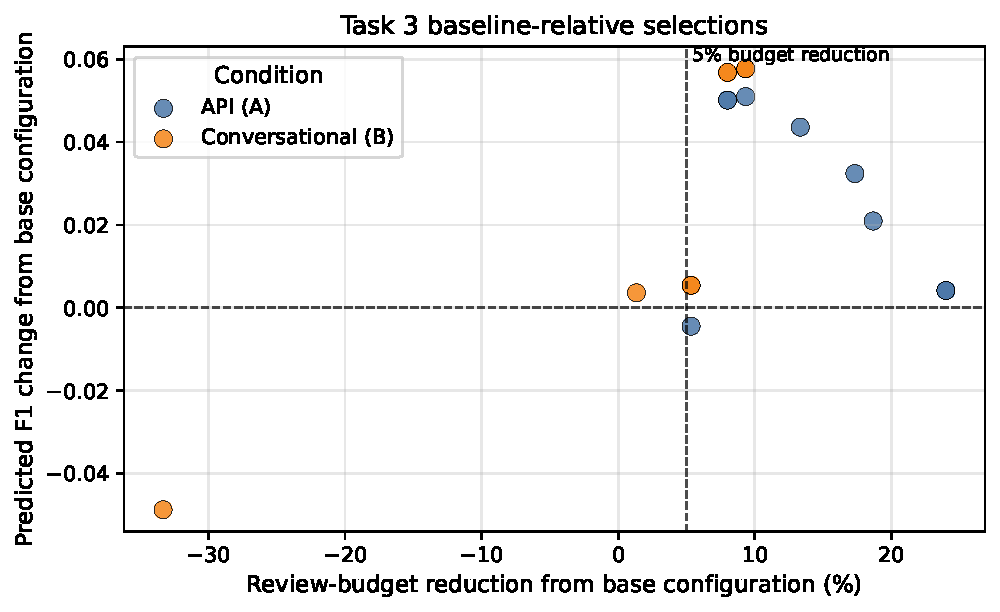
\includegraphics[width=\columnwidth]{fig_user_study_task3_quality_budget_tradeoff.pdf}
    \caption{Task~3 quality--effort trade-off relative to the base configuration.}
    \label{fig:user-study-task3}
\end{figure}

\paragraph{Questionnaire}
Condition B scored higher on four of the five post-task questionnaire
items. The largest raw difference was for comparing options (B: 4.36
compared with A: 3.44, Mann-Whitney $p = 0.10$), followed by
identifying valid F1 configurations (4.91 compared with 4.44,
$p = 0.08$) and understanding trade-offs (3.91 compared with 3.56,
$p = 0.44$); the two conditions were close on checking constraints
(4.18 compared with 4.00, $p = 0.45$) and on using the provided tool,
where condition A was marginally higher (4.33 compared with 4.27,
$p = 1.00$). After Holm correction for five simultaneous tests, no item
reaches significance. All differences should be treated as descriptive
indicators of perceived usability rather than as reliable effect
estimates, given the sample sizes ($n_A = 9$, $n_B = 11$) and the
between-subjects design.

\paragraph{Over-reliance proxies}
Over-reliance was not measured directly; three descriptive proxies from
the condition-B logs bound it. Of the $32$ answers for which the
interface displayed a ``balanced choice'' recommendation ($35$
selections in total), $16$ followed it; all $35$ selected options were
retrieved logged trials, because retrieval answered every query; and all four invalid selections were made while the interface stated
that every displayed option met the parsed constraints. Three trace to a fluently confirmed parse that was incomplete (two Task-1 parses dropped the upper training-fraction bound) or unfaithful (one Task-3 parse); the fourth participant rewrote the $5\%$ reduction as an absolute budget that reduced it by less. In all four the interface confirmed the parsed query rather than the task.

\subsection{Qualitative Analysis of Participant Justifications}
\label{subsec:justification-analysis}

To complement the quantitative results we analysed the short written
justifications qualitatively, using a large language model as an
automated judge \cite{zheng_judging_2023} to reduce confirmation bias.
The model was Claude Opus~5 (Anthropic), used through its interactive interface in a single session in July 2026 (the interface exposes no model snapshot identifier); the complete structured prompt and the
anonymised comment bundle it received are released in the archive
(\path{user_study/tables/qualitative_comments/}). The prompt requested
descriptive analysis of attribute references, trade-off reasoning,
condition differences, Task-3 what-if reasoning, and over-reliance on
predicted F1, without overclaiming or identifying participants. Because
the interactive interface does not expose a sampling temperature, the
output is not bit-reproducible; the authors reviewed the summary for
factual consistency with the raw comments, and the observations below
are the model's reading of the comments, not measurements.

\paragraph{Findings}
Participants grounded choices in a few attributes (predicted F1, review
budget, less often training fraction and corruption level) with brief,
outcome-oriented justifications; a minority reasoned about trade-offs.
Condition-A participants anchored on F1 maximisation, condition-B
participants more often cited named options and the interface's
``balanced compromise'' framing. Task~3 elicited the most varied
justifications: the relative constraint led to invalid selections
believed to be valid, and several participants in both conditions
optimised absolute F1 or the absolute budget rather than the percentage
reduction. Tentative design implications: scaffold secondary metrics as
first-class criteria, give baseline-relative constraints continuously
updated satisfaction feedback, and use evaluative option labels with
care, since they may be accepted uncritically.

% =======================================================================
\section{Discussion}
\label{sec:discussion}
% =======================================================================

\subsection{Interpreting the Two-Dataset Technical Results}
\label{subsec:discussion-technical}

The paired evaluation establishes a production result and the two
conditions needed to trust it. On Proditec, all 24 recommendations meet
their target after retraining (mean confirmed F1 $0.879$, gap $-0.007$,
AUROC $0.976$). On MVTec, all 24 meet the target under the per-category
protocol (mean $0.787$, gap $-0.023$); a single pooled threshold over the same models' concatenated scores measures a different quantity and shows an apparent gap of $-0.24$. The first condition is therefore that confirmation follows the optimisation objective. The second is that surrogate fidelity is not
the same as HPO value: on these four MVTec categories, in the single run available, an untuned reference beats the HPO optimum and every recommendation at the HPO
budget ($0.867$ against $0.786$ and $0.787$), because the review-budget
objective at $\beta \approx 0.5$ and $70\%$ prevalence is bounded at
$0.83$ and flat across the top of the log. A surrogate that faithfully reproduces such an objective faithfully reproduces its blind spot, so MVTec supports the protocol and objective lessons rather than a claim of recommendation value.
Per-category AUROC of $0.913$ against pooled $0.527$ shows,
independently of any threshold, that pooling categories with
incommensurable score scales damages the global ranking. The two
datasets use different objectives, prevalences ($0.70$ and $0.345$),
log sizes, and anchors, so their comparison is descriptive, not
controlled. 

\subsection{Implications for Operator-Centred HPO}
\label{subsec:discussion-operator}

The user evaluation concerns the complete study-time workflow.
Technically literate non-specialists produced high task validity in
both conditions; condition-B participants rated ease of comparing
options higher (4.36 against 3.44), but no item survives Holm
correction, assignment was by time block, and both conditions presented
tabular results, so the difference is descriptive and cannot be
attributed to conversational interaction rather than to the added
summary and option labels. Because the study-time parser reached $15\%$
exact accuracy on the fields the interface uses and $25$ of $72$ live parses were incomplete or unfaithful ($17$ visibly, $8$ as fluent lists), task success reflects the combined interaction (repair, anchoring, presentation, iteration) rather than one-shot parsing, and three of the four invalid condition-B selections trace to parses the interface fluently confirmed. Baseline-relative requirements drove condition-B
attempt counts ($3.1$ per Task-3 answer against $1.4$--$1.8$ on the
absolute tasks; condition-A counts measure API invocations and are not
comparable). The direct remedy is to treat relative constraints as
first-class objects and resolve their arithmetic deterministically; the
revised parser and production operators are the next evaluation
setting.

\subsection{Limitations}
\label{subsec:limitations}

\paragraph{Scope of datasets and task}
The evaluation covers four MVTec categories and one production use case
on a single architecture with a fixed configuration space; two datasets
do not establish that the pooled score-scale pathology, seen on MVTec
and not on Proditec, generalises to other multi-category or
single-product deployments.

\paragraph{Confirmation coverage}
Confirmation covers the 24 primary candidates per dataset under three
seeds, the 12 retrieval-comparison candidates, the 60 anchor-sweep candidates, 96 logged trials (48 per dataset), and the MVTec no-HPO reference, but the anchor sweep, the retrieval comparison, and the reference use a single seed,
and the Proditec recommendations all lie in a small neighbourhood of the
best trial, so local fidelity is well tested and fidelity far from the
anchor is tested only by the sweep.

\paragraph{Language-model parsing reliability}
The released front-end parses 60\% of labelled utterances exactly
(77\% among accepted outputs) and falls back on 22.5\%; the study-time front-end parsed 15\% exactly on the fields the interface uses (2.5\% including the alternative count, which the interface fixed) and, when it returned schema-valid JSON, was wrong on those fields in 12 of 18 cases. Relative constraints fail entirely
at the parser level in both. This is an addressable architecture
limitation rather than a reason to delegate arithmetic to a larger
language model: the parser can extract the quantity and reference
field, after which deterministic code computes the bound. The
user-study results apply to the complete workflow, including repair,
anchoring, overlay, and iteration, rather than to one-shot parsing, and incomplete or unfaithful parses that are fluently confirmed (8 of 72 live attempts) are the safety-relevant failure mode of that workflow.

\paragraph{User-study population}
The participants were computer-science master's students, a proxy for
reasoning about model quality, training data, and thresholds, not
industrial inspection operators, who carry domain priors about defects
and inspection cost, face real consequences for a wrong configuration,
and may weigh review effort differently. The study therefore supports
usability claims for technically literate non-specialists and
motivates, rather than substitutes for, a planned operator-population
study.

\paragraph{User-study scale and design}
The study is exploratory: 22 participants across two conditions
assigned by time block, descriptive statistics only, condition-specific
logging of attempt counts, voluntary questionnaire completion with a
mild imbalance ($n_A = 9$, $n_B = 11$), no demographic covariates, and
no questionnaire item surviving Holm correction. The results are design
evidence, not confirmatory effect estimates.

\paragraph{Presentation confound and over-reliance}
Condition B differs from condition A in input modality, in the textual
summary, and in evaluative option labels, so the questionnaire
differences cannot be attributed to conversational interaction alone.
Over-reliance was not measured; the proxies of
Section~\ref{subsec:user-study-results} (half of the selections
following the recommended option; all invalid selections made under a
fluent all-constraints-met message) motivate a dedicated study with
manipulated recommendation quality.

\paragraph{HPO value and the untuned reference}
On MVTec, in the single run available, an untuned PatchCore reference outperforms the HPO optimum and all recommendations at the HPO budget (Section~\ref{subsec:gap-diagnosis}).
On Proditec no reference run exists, so the positive result there
(24/24 in band, all candidates near the best logged trial, whose logged
F1 of $0.908$ re-measures at $0.904$) shows that surrogate and retrieval
return what the log already contains, $43\%$ of which lies in the
requested band, not that HPO or the recommendations beat an untuned reference. The
framework cannot repair an objective whose top is a plateau bounded by
the operating-point rule; recommendations drawn from such a log should
be benchmarked against an untuned reference configuration before deployment.

\paragraph{No surrogate support indicator}
The interface gives no per-candidate reliability signal. It already
computes mixed-type distance to the factual and logged status, so it
could flag weakly supported candidates and recommend confirmation.
Logged status alone is insufficient: the primary MVTec \textsc{LogTopK}
candidates are logged trials and were confirmed only once the protocol
was corrected, and the anchor-sweep failures were marginal logged and
generated candidates alike. A useful signal must combine support, local
error, seed variability, and target stability; such a signal is not
part of the evaluated system, and a Gaussian-process surrogate with
calibrated intervals (Section~\ref{subsec:surrogate-fidelity}) is one
route to it.

\paragraph{Explanation faithfulness}
The released interface renders explanations deterministically from the
structured payload and appends a note that the text is generated
automatically. The study-time interface additionally rephrased that
template with the language model, and those texts were not audited at
study time. A post-hoc numeric audit of the 51 polished explanations
shown to participants found that 49 reproduced every number of the
template exactly; two (both in Task~3) altered the figures, one omitting
four small differences and one rendering a budget difference of $0.030$
as $0.3$ and omitting two others. The audit covers numbers only, not
comparative wording, so a mechanically checkable faithfulness suite
(agreement with the candidate table, correct constraint status, tie
preservation, no unsupported trade-offs) remains planned, and
language-model rephrasing should be regarded as unverified presentation
until it exists.

\paragraph{Energy measurement}
No power telemetry was collected; runtime is reported in
Section~\ref{subsec:compute-cost}, but no energy or CO$_2$ saving is
claimed.

% =======================================================================
\section{Conclusion}
\label{sec:conclusion}
% =======================================================================

This paper presented CF-XHPO, a framework that turns HPO logs into
operator-centred what-if guidance for industrial visual anomaly
detection by combining surrogate modelling, constrained retrieval,
counterfactual generation, deterministic query validation, and a
conversational interface. Over 500 PatchCore retrainings confirm the evaluation. All 48 primary recommendations
satisfy their surrogate-level queries and all 48 meet their targets after retraining (three-seed mean confirmed F1) under the protocol of the optimisation objective
(mean confirmed F1 $0.879$ on Proditec and $0.787$ on MVTec, gaps
$-0.007$ and $-0.023$).

The evaluation also establishes how such guidance should be validated.
A single pooled threshold over four categories measures a different quantity from the objective and shows an apparent gap of $-0.24$ for the same models; under the per-category protocol the surrogate predicts
its target to within $0.001$. Pooling categories with incommensurable
score scales reduces AUROC from $0.913$ to $0.527$, so heterogeneous
deployments need per-category thresholds. And surrogate fidelity is not
HPO value: the MVTec objective is degenerate at the HPO budget (F1
bounded at $0.83$, the top tenth of the log within $0.80$--$0.82$) and
an untuned reference reaches $0.867$ in a single run, above the HPO optimum and every recommendation, so MVTec supports the protocol and objective lessons
rather than a claim of recommendation value, while Proditec, where
$43\%$ of the log already lies in band and no reference was run, shows
that retrieval returns what the log contains. The policy is to match the
confirmation protocol to the objective, report threshold-free AUROC and
the operating-point F1 bounds next to review-budget F1, benchmark
against the untuned reference and the in-band share of the log, and
confirm final recommendations with the underlying model.

Constrained retrieval matches off-log generation and a filter-and-sort baseline on the tested logs, so the surrogate is not needed for retrieval when the log is dense, motivating a retrieve-first policy, and the interaction overhead amortises from
about three alternatives upward with a CPU language model. Both study
workflows supported high task validity; questionnaire differences in
favour of the conversational condition are descriptive and confounded
with presentation, and the result was reached despite a parser that produced the exact query for $15\%$ of benchmark utterances on the fields the interface uses and parsed $25$ of $72$ live requests incompletely or unfaithfully, eight of them shown as fluent lists. CF-XHPO is therefore
not a replacement for model evaluation but a screening and
decision-support layer over trials an HPO process has already produced,
whose value is bounded by the quality of that process. Future work will
resolve relative constraints deterministically, surface a support
indicator distinguishing confirmed, logged, and generated candidates,
add a mechanically checked faithfulness suite for explanations, repeat
the user evaluation with the released parser and with production
operators, and extend confirmation across seeds, anchors, categories,
and further industrial use cases.

% =======================================================================
\section*{Declaration of competing interest}
The authors declare that they have no known competing financial
interests or personal relationships that could have appeared to
influence the work reported in this paper.

\section*{Declaration of Generative AI and AI-assisted Technologies}
During preparation, the authors used Claude Opus 5 (Anthropic) to
support the implementation and analysis of experiments; all analyses
were verified by the authors against the released code and results
before inclusion in the manuscript. Claude Opus 5 was also used to
support the qualitative summarisation of anonymised participant
comments (Section~\ref{subsec:justification-analysis}) and to improve
language and readability. The authors reviewed and edited all output
and take full responsibility for the publication.

\section*{Data availability}
The MVTec~AD benchmark is publicly available
\cite{bergmann_mvtec_2019}; the Proditec images are proprietary and
cannot be shared. All code and derived data (optimisation logs,
preprocessing and surrogate code, candidate-production and retrieval
implementations, the twelve-query suite, parser prompts and the
40-utterance evaluation set, per-candidate confirmation results, the
review notebooks R00--R07 with their frozen result tables, seeds, and a
dependency list), together with a live demonstration of the interface,
are publicly archived; the links are withheld for double-blind review,
are available to the editor and reviewers on request, and will be
restored in the camera-ready version.

\bibliographystyle{elsarticle-num}
\bibliography{references}

\end{document}